% Created 2019-12-04 Wed 17:10
% Intended LaTeX compiler: pdflatex
\documentclass[10pt, compress, aspectratio=169, xcolor={table,usenames,dvipsnames}]{beamer}

\usepackage{booktabs}
\mode<beamer>{\usetheme[numbering=fraction, progressbar=none, titleformat=smallcaps, sectionpage=none]{metropolis}}
\usepackage{sourcecodepro}
\usepackage{booktabs}
\usepackage{array}
\usepackage{listings}
\usepackage{graphicx}
\usepackage[english]{babel}
\usepackage[scale=2]{ccicons}
\usepackage{url}
\usepackage{relsize}
\usepackage{amsmath}
\usepackage{bm}
\usepackage{wasysym}
\usepackage{ragged2e}
\usepackage{textcomp}
\usepackage{pgfplots}
\usepackage{multirow}
\usepgfplotslibrary{dateplot}
\definecolor{Base}{HTML}{191F26}
\definecolor{Highlight}{HTML}{ffda99}
\definecolor{Accent}{HTML}{bb0300}
\setbeamercolor{alerted text}{fg=Accent}
\setbeamercolor{frametitle}{bg=Base}
\setbeamercolor{normal text}{bg=black!2,fg=Base}
\setsansfont[BoldFont={Source Sans Pro Semibold},Numbers={OldStyle}]{Source Sans Pro}
\lstdefinelanguage{Julia}%
{morekeywords={abstract,struct,break,case,catch,const,continue,do,else,elseif,%
end,export,false,for,function,immutable,mutable,using,import,importall,if,in,%
macro,module,quote,return,switch,true,try,catch,type,typealias,%
while,<:,+,-,::,/},%
sensitive=true,%
alsoother={$},%
morecomment=[l]\#,%
morecomment=[n]{\#=}{=\#},%
morestring=[s]{"}{"},%
morestring=[m]{'}{'},%
}[keywords,comments,strings]%
\lstset{ %
backgroundcolor={},
basicstyle=\ttfamily\scriptsize,
breakatwhitespace=true,
breaklines=true,
captionpos=n,
commentstyle=\color{Accent},
extendedchars=true,
frame=n,
keywordstyle=\color{Accent},
language=R,
rulecolor=\color{black},
showspaces=false,
showstringspaces=false,
showtabs=false,
stepnumber=2,
stringstyle=\color{gray},
tabsize=2,
}
\renewcommand*{\UrlFont}{\ttfamily\smaller\relax}
\graphicspath{{../../img/}}
\addtobeamertemplate{block begin}{}{\justifying}
\usetheme{default}
\author{ \footnotesize \textbf{\alert{Pedro Bruel$^{*}$}},  Steven Quinito Masnada, Brice Videau, Arnaud Legrand, Jean-Marc Vincent, Alfredo Goldman}
\date{ \scriptsize \textit{phrb@ime.usp.br} \\[1em] \textit{Universidade de São Paulo, Brazil} \\ \textit{Université Grenoble Alpes, France}}
\title{Autotuning under Tight Budget Constraints:  \\ An Experimental Design Approach}
\hypersetup{
 pdfauthor={ \footnotesize \textbf{\alert{Pedro Bruel$^{*}$}},  Steven Quinito Masnada, Brice Videau, Arnaud Legrand, Jean-Marc Vincent, Alfredo Goldman},
 pdftitle={Autotuning under Tight Budget Constraints:  \\ An Experimental Design Approach},
 pdfkeywords={},
 pdfsubject={},
 pdfcreator={Emacs 26.3 (Org mode 9.2.5)},
 pdflang={English}}
\begin{document}

\maketitle

\section{Autotuning}
\label{sec:org43a8f42}
\begin{frame}[label={sec:orgb80100e}]{Autotuning: Optimizing Program Configurations}
\begin{columns}
\begin{column}{0.5\columnwidth}
\begin{block}{Architectures for High Performance Computing}
\begin{center}
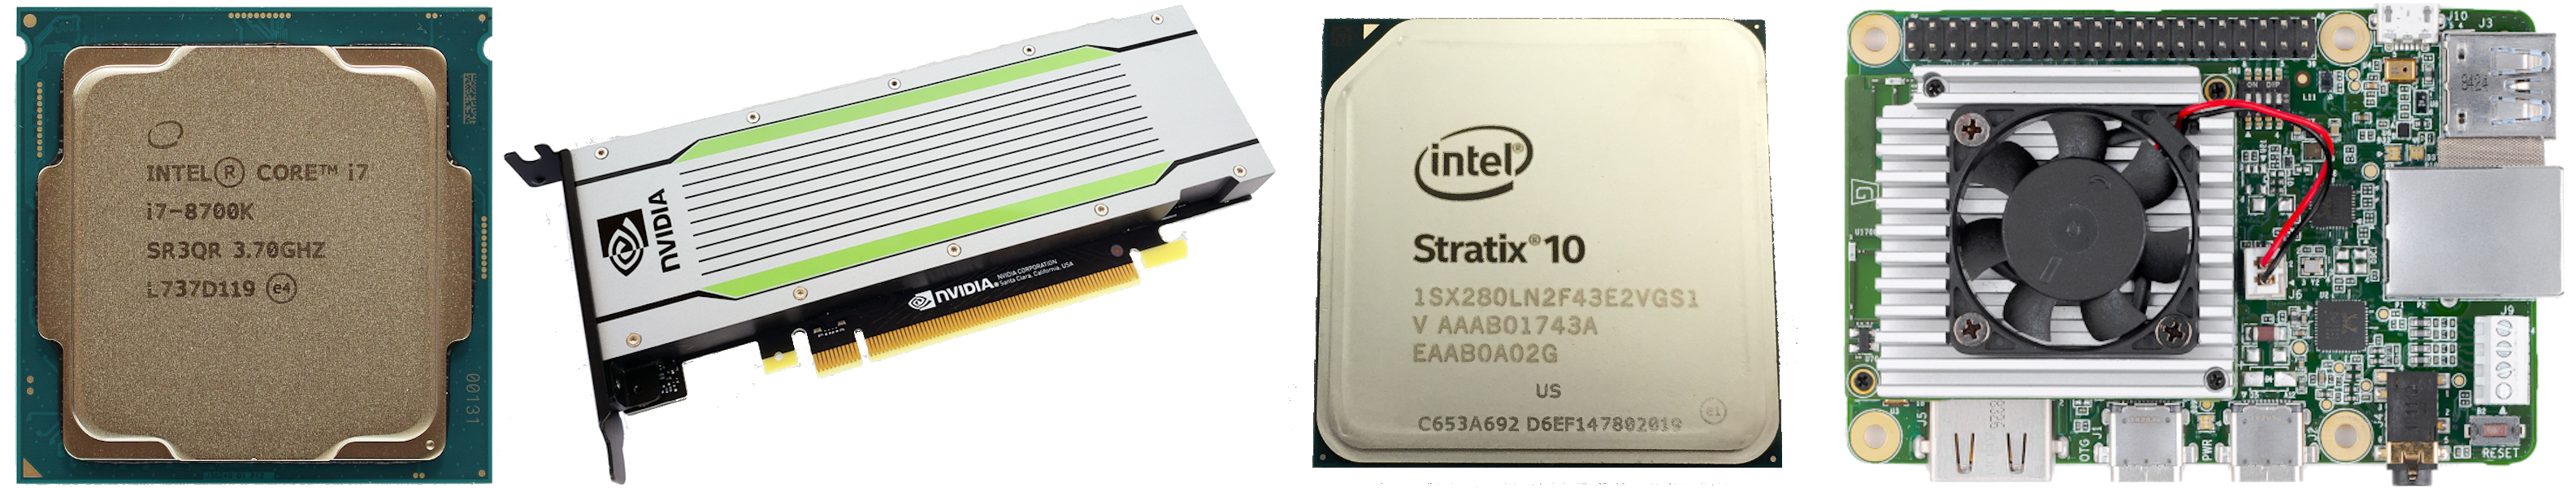
\includegraphics[width=\columnwidth]{../../../img/architectures_2.png}
\end{center}

How to write \alert{efficient code} for each of these?

\begin{block}{Autotuning}
\vspace{.2cm}

The process of automatically finding a \mbox{\alert{configuration}} of a program
that optimizes an \mbox{\alert{objective}}
\end{block}
\end{block}
\end{column}

\begin{column}{0.5\columnwidth}
\begin{block}{Configurations}
\begin{itemize}
\item Algorithms
\begin{itemize}
\item Sorting, encoding, \(\dots\)
\end{itemize}
\item Implementations
\begin{itemize}
\item Code transformation, libraries, \(\dots\)
\end{itemize}
\item Context-specific parameters
\begin{itemize}
\item Compilers, kernels, \(\dots\)
\end{itemize}
\end{itemize}

\begin{block}{Objectives}
\begin{itemize}
\item Execution time
\item Resource consumption
\item Binary size
\item \(\dots\)
\end{itemize}
\end{block}
\end{block}
\end{column}
\end{columns}
\end{frame}

\begin{frame}[label={sec:org40fb639}]{Autotuning: Search Spaces}
\begin{columns}
\begin{column}{0.4\columnwidth}
\begin{block}{Search Spaces}
\vspace{.2cm}

Represent the \alert{effect} of all possible
configurations on target objectives

Can be difficult to explore, with multiple \mbox{\alert{local optima}}
and \mbox{\alert{undefined}} \mbox{\alert{regions}}
\end{block}
\end{column}

\begin{column}{0.6\columnwidth}
\begin{center}
\begin{center}
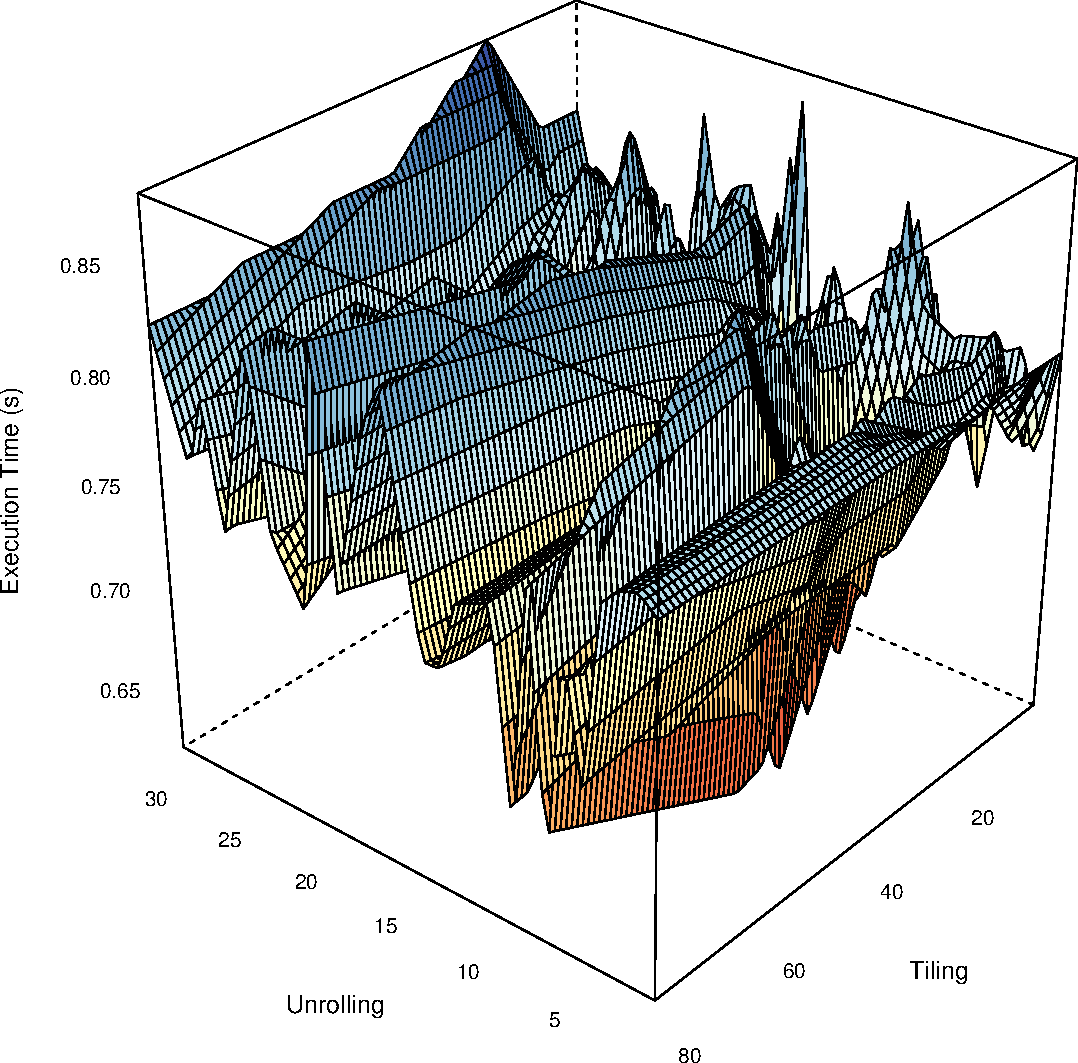
\includegraphics[width=.8\columnwidth]{../../../img/bicgkernel_averaged_search_space.pdf}
\end{center}
\end{center}

\center{\footnotesize
Unrolling, tiling and performance for a \alert{biconjugate gradient} kernel
}
\end{column}
\end{columns}
\end{frame}

\begin{frame}[label={sec:org850d0ae}]{Autotuning: High-Dimensional Search Spaces}
\begin{block}{1. \alert{Combinatorial Explosion \& Sampling}}
\begin{itemize}
\item 10 boolean parameters generate \(2^{10}\) combinations
\item 10 continuous parameters in \([0, 1]\)  need \((10^{2})^{10}\) points to cover with
spacing \(10^{-2}\)
\item Sampling a hypercube covers its shell
\end{itemize}
\end{block}

\begin{columns}
\begin{column}{0.5\columnwidth}
\begin{block}{2. \alert{Geometry}}
\begin{itemize}
\item Mixing discrete and continous factors
\item ``Smoothness''
\item Interactions
\item Constraints
\item Undefined regions
\end{itemize}
\end{block}
\end{column}

\begin{column}{0.5\columnwidth}
\begin{block}{3. \alert{Measurement Time}}
\begin{itemize}
\item Compile time:
\begin{itemize}
\item FPGA applications
\item Hardware/Software codesign
\end{itemize}
\item Execution time:
\begin{itemize}
\item Simulations
\item Neural network training
\end{itemize}
\end{itemize}
\end{block}
\end{column}
\end{columns}
\end{frame}

\begin{frame}[label={sec:org63fe464}]{Autotuning: Approaches}
\begin{columns}
\begin{column}{0.5\columnwidth}
\begin{block}{Several Approaches}
\footnotesize
\begin{itemize}
\item \colorbox{red!25}{Exhaustive}
\item \colorbox{green!25}{Meta-Heuristics}
\item \colorbox{cyan!25}{Machine Learning}
\end{itemize}
\normalsize

\vspace{-.4cm}

\begin{table}
    \centering
    \scriptsize
    \begin{tabular}{@{}lll@{}}
        \toprule
        System & Domain & Approach \\ \midrule
        \rowcolor{red!25} ATLAS & Dense Linear Algebra & Exhaustive\\ \addlinespace
        \rowcolor{green!25} INSIEME & Compiler & Genetic Algorithm \\
        \rowcolor{green!25} Active Harmony & Runtime & Nelder-Mead \\
        \rowcolor{green!25} ParamILS & Domain-Agnostic & Stochastic Local Search \\
        \rowcolor{green!25} OPAL & Domain-Agnostic & Direct Search \\
        \rowcolor{green!25} OpenTuner & Domain-Agnostic & Ensemble \\ \addlinespace
        \rowcolor{cyan!25} MILEPOST GCC & Compiler & Machine Learning \\
        \rowcolor{cyan!25} Apollo & GPU kernels & Decision Trees \\ \addlinespace
        \bottomrule
    \end{tabular}
\end{table}

\end{block}
\end{column}

\begin{column}{0.5\columnwidth}
\begin{block}{Core Assumptions:}
\begin{itemize}
\item A large number of function evaluations
\item Good solutions are reachable
\item Seach space ``smoothness''
\end{itemize}
\begin{block}{After Optimization:}
\begin{itemize}
\item \alert{Learn ``nothing''} about the search space
\item \alert{Can't explain} why optimizations work
\end{itemize}
\end{block}
\begin{block}{We propose using:}
\begin{itemize}
\item \alert{Experimental Design} (\alert{ED})
\end{itemize}
\end{block}
\end{block}
\end{column}
\end{columns}
\end{frame}
\section{Experimental Design}
\label{sec:org659d508}
\begin{frame}[label={sec:orga0e1381}]{Experimental Design: An Example on Agriculture}
\begin{columns}
\begin{column}{0.55\columnwidth}
\begin{center}
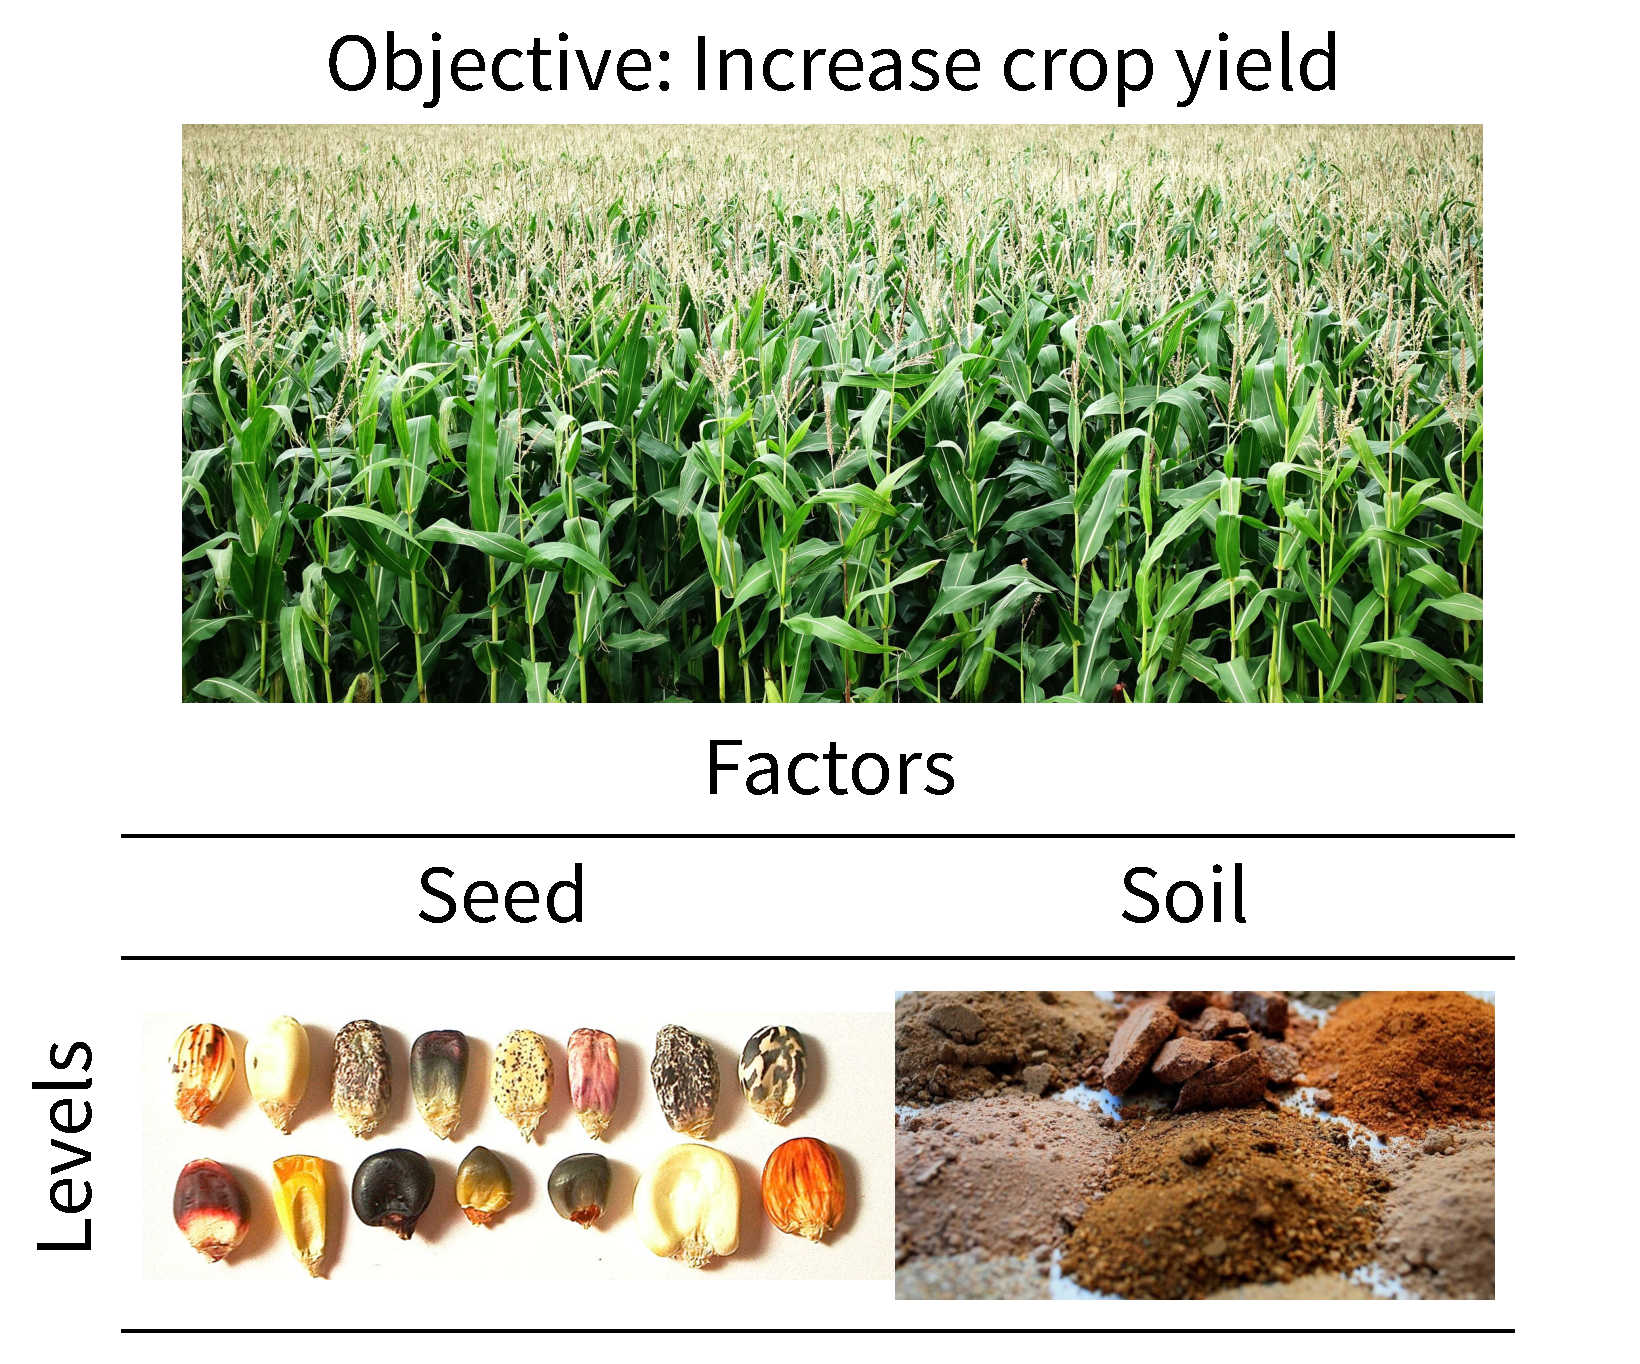
\includegraphics[width=.99\columnwidth]{../../../img/crop_yield_doe_example.pdf}
\end{center}
\end{column}
\begin{column}{0.45\columnwidth}
\begin{block}{Testing all combinations is \alert{inviable}}
\begin{block}{Which combinations to test?}
\begin{itemize}
\item ED provides a selection method
\item \colorbox{Highlight}{\alert{Parsimony}: decreases experiments}
\end{itemize}
\end{block}

\begin{block}{Which is the best combination?}
\begin{itemize}
\item ED provides an analysis method
\item \colorbox{Highlight}{\alert{Transparency}: use statistical tests}
\end{itemize}
\end{block}
\end{block}
\end{column}
\end{columns}
\end{frame}

\begin{frame}[label={sec:org95f56c5}]{Experimental Design}
\begin{columns}
\begin{column}{0.5\columnwidth}
\begin{block}{Terminology}
\begin{itemize}
\item Factors: program parameters
\item Levels: possible factor values
\item Experiment: setting each factor to a level
\item Design: a selection of experiments to run
\item \uncover<2>{Performance model: guides selection}
\end{itemize}

\begin{block}{Analyzing Results Enable:}
\begin{itemize}
\item Identifying \alert{significant factors}
\item Investigating possible \alert{models}
\item Finding candidates for \alert{further experimentation}
\end{itemize}
\end{block}
\end{block}
\end{column}

\begin{column}{0.5\columnwidth}
\begin{block}{Example}
\vspace{-.2cm}
\begin{center}

A minimal screening design for \(7\) 2-level factors:

\end{center}
\vspace{-.2cm}

\begin{table}[]
    \centering
    \begin{tabular}{@{\kern\tabcolsep}cccccccc@{\kern\tabcolsep}}
        \toprule
        Run & A & B & C & D & E & F & G \\ \midrule
        \cellcolor{gray!18}1 & \cellcolor{green!25}1 & \cellcolor{red!25}-1 & \cellcolor{green!25}1 & \cellcolor{red!25}-1 & \cellcolor{red!25}-1 & \cellcolor{green!25}1 & \cellcolor{green!25}1 \\
        \cellcolor{gray!18}2 & \cellcolor{green!25}1 & \cellcolor{green!25}1 & \cellcolor{green!25}1 & \cellcolor{red!25}-1 & \cellcolor{green!25}1 & \cellcolor{red!25}-1 & \cellcolor{red!25}-1 \\
        \cellcolor{gray!18}3 & \cellcolor{red!25}-1 & \cellcolor{green!25}1 & \cellcolor{red!25}-1 & \cellcolor{red!25}-1 & \cellcolor{green!25}1 & \cellcolor{green!25}1 & \cellcolor{green!25}1 \\
        \cellcolor{gray!18}4 & \cellcolor{red!25}-1 & \cellcolor{green!25}1 & \cellcolor{green!25}1 & \cellcolor{green!25}1 & \cellcolor{red!25}-1 & \cellcolor{green!25}1 & \cellcolor{red!25}-1 \\
        \cellcolor{gray!18}5 & \cellcolor{green!25}1 & \cellcolor{red!25}-1 & \cellcolor{red!25}-1 & \cellcolor{green!25}1 & \cellcolor{green!25}1 & \cellcolor{green!25}1 & \cellcolor{red!25}-1 \\
        \cellcolor{gray!18}6 & \cellcolor{green!25}1 & \cellcolor{green!25}1 & \cellcolor{red!25}-1 & \cellcolor{green!25}1 & \cellcolor{red!25}-1 & \cellcolor{red!25}-1 & \cellcolor{green!25}1 \\
        \cellcolor{gray!18}7 & \cellcolor{red!25}-1 & \cellcolor{red!25}-1 & \cellcolor{green!25}1 & \cellcolor{green!25}1 & \cellcolor{green!25}1 & \cellcolor{red!25}-1 & \cellcolor{green!25}1 \\
        \cellcolor{gray!18}8 & \cellcolor{red!25}-1 & \cellcolor{red!25}-1 & \cellcolor{red!25}-1 & \cellcolor{red!25}-1 & \cellcolor{red!25}-1 & \cellcolor{red!25}-1 & \cellcolor{red!25}-1  \\ \bottomrule
    \end{tabular}
\end{table}

\vspace{-.2cm}

\uncover<2>{$$response = \theta{} + \alpha{}A + \beta{}B + \gamma{}C + \dots$$}
\end{block}
\end{column}
\end{columns}
\end{frame}

\begin{frame}[label={sec:org8d35656}]{Applying Experimental Design to Autotuning}
\begin{columns}
\begin{column}{0.45\columnwidth}
\begin{block}{Design Requirements}
\begin{itemize}
\item Support a large number of factors (\alert{Combinatorial Explosion})
\item Maximize the amount of information (\alert{Sampling})
\item Support mixing factor types (\alert{Geometry})
\item Minimize function evaluations (\alert{Measurement Time})
\end{itemize}
\end{block}
\end{column}

\begin{column}{0.55\columnwidth}
\begin{block}{Initial Experimental Design Approach}
\begin{itemize}
\item D-Optimal designs
\begin{itemize}
\item Flexible
\item Minimize variance of coefficient estimators
\item Support different factor types
\end{itemize}
\item Linear model and analysis of variance (ANOVA)
\item User input to guide optimization
\item \colorbox{Highlight}{\alert{Parsimony} \& \alert{Transparency}}
\end{itemize}

\begin{block}{Validation}
\begin{itemize}
\item Code transformation:
\begin{itemize}
\item GPU Laplacian kernel
\item HPC kernels from the SPAPT benchmark
\end{itemize}
\end{itemize}
\end{block}
\end{block}
\end{column}
\end{columns}
\end{frame}

\begin{frame}[label={sec:orge4b90a0}]{D-Optimal Designs: A Simple Example in R}
\begin{columns}
\begin{column}{0.5\columnwidth}
\begin{block}{Search Space}
% \(\mathbf{X} = \{x_1 = \{1, 2, 3, 4, 5\}, x_2 = \{"A", "B", "C"\}\}\)
\begin{itemize}
\item Factors \& Levels:
\begin{align*}
\mathbf{X} = (x_1 = & \; (1, 2, 3, 4, 5), \\
x_2 = & \; (``A", ``B", ``C"))
\end{align*}
\item 15 possible experiments
\item Model: \(\mathbf{Y} = \mathbf{X}\bm{\beta} + \bm{\varepsilon}\)
\end{itemize}
\end{block}
\end{column}

\begin{column}{0.5\columnwidth}
\begin{block}{Ordinary Least Squares Estimator \(\bm{\hat{\beta}}\)}
\begin{center}
\begin{equation*}
\bm{\hat{\beta}} = \left(\bm{X}^{\intercal}\bm{X}\right)^{-1}\bm{X}^{\intercal}\bm{Y}
\end{equation*}
\end{center}

\begin{center}
\colorbox{Highlight}{\parbox[c]{0.8\columnwidth}{\centering The \alert{variance} of $\bm{\hat{\beta}}$ is proportional to \\
    the \alert{covariance matrix} $\left(\bm{X}^{\intercal}\bm{X}\right)^{-1}$}}
\end{center}
\end{block}
\end{column}
\end{columns}
\end{frame}

\begin{frame}[label={sec:org757a939},fragile]{D-Optimal Designs: A Simple Example in R}
 \begin{columns}
\begin{column}{0.7\columnwidth}
\begin{block}{Source code in \texttt{R}}
\vspace{-.2cm}

\lstset{language=r,label= ,caption= ,captionpos=b,numbers=none}
\begin{lstlisting}
library(DoE.base)
library(AlgDesign)

samples <- fac.design(nfactors = 2,
                      nlevels = c(5, 3),
                      factor.names = list(x1 = 1:5,
                                          x2 = c("A", "B", "C")))

output <- optFederov(~ x1 + x2,
                     samples,
                     nTrials = 7)
\end{lstlisting}

\begin{block}{Optimality Criteria}
\begin{itemize}
\item \alert{D} (determinant): minimizes generalized variance of \(\bm{\hat{\beta}}\)
\item \alert{A} (trace): average variance of \(\bm{\hat{\beta}}\)
\item \dots{}
\end{itemize}
\end{block}
\end{block}
\end{column}


\begin{column}{0.3\columnwidth}
\begin{block}{Output}
\vspace{-.2cm}
\scriptsize

\begin{verbatim}
$D
[1] 0.1797856

$design
   x1 x2
1   1  C
2   1  A
3   5  A
5   3  B
6   3  A
12  2  A
14  4  B
\end{verbatim}


\normalsize
\end{block}
\end{column}
\end{columns}
\end{frame}

\begin{frame}[label={sec:org3486c76}]{Comparing Sampling Strategies}
\begin{center}
\begin{center}
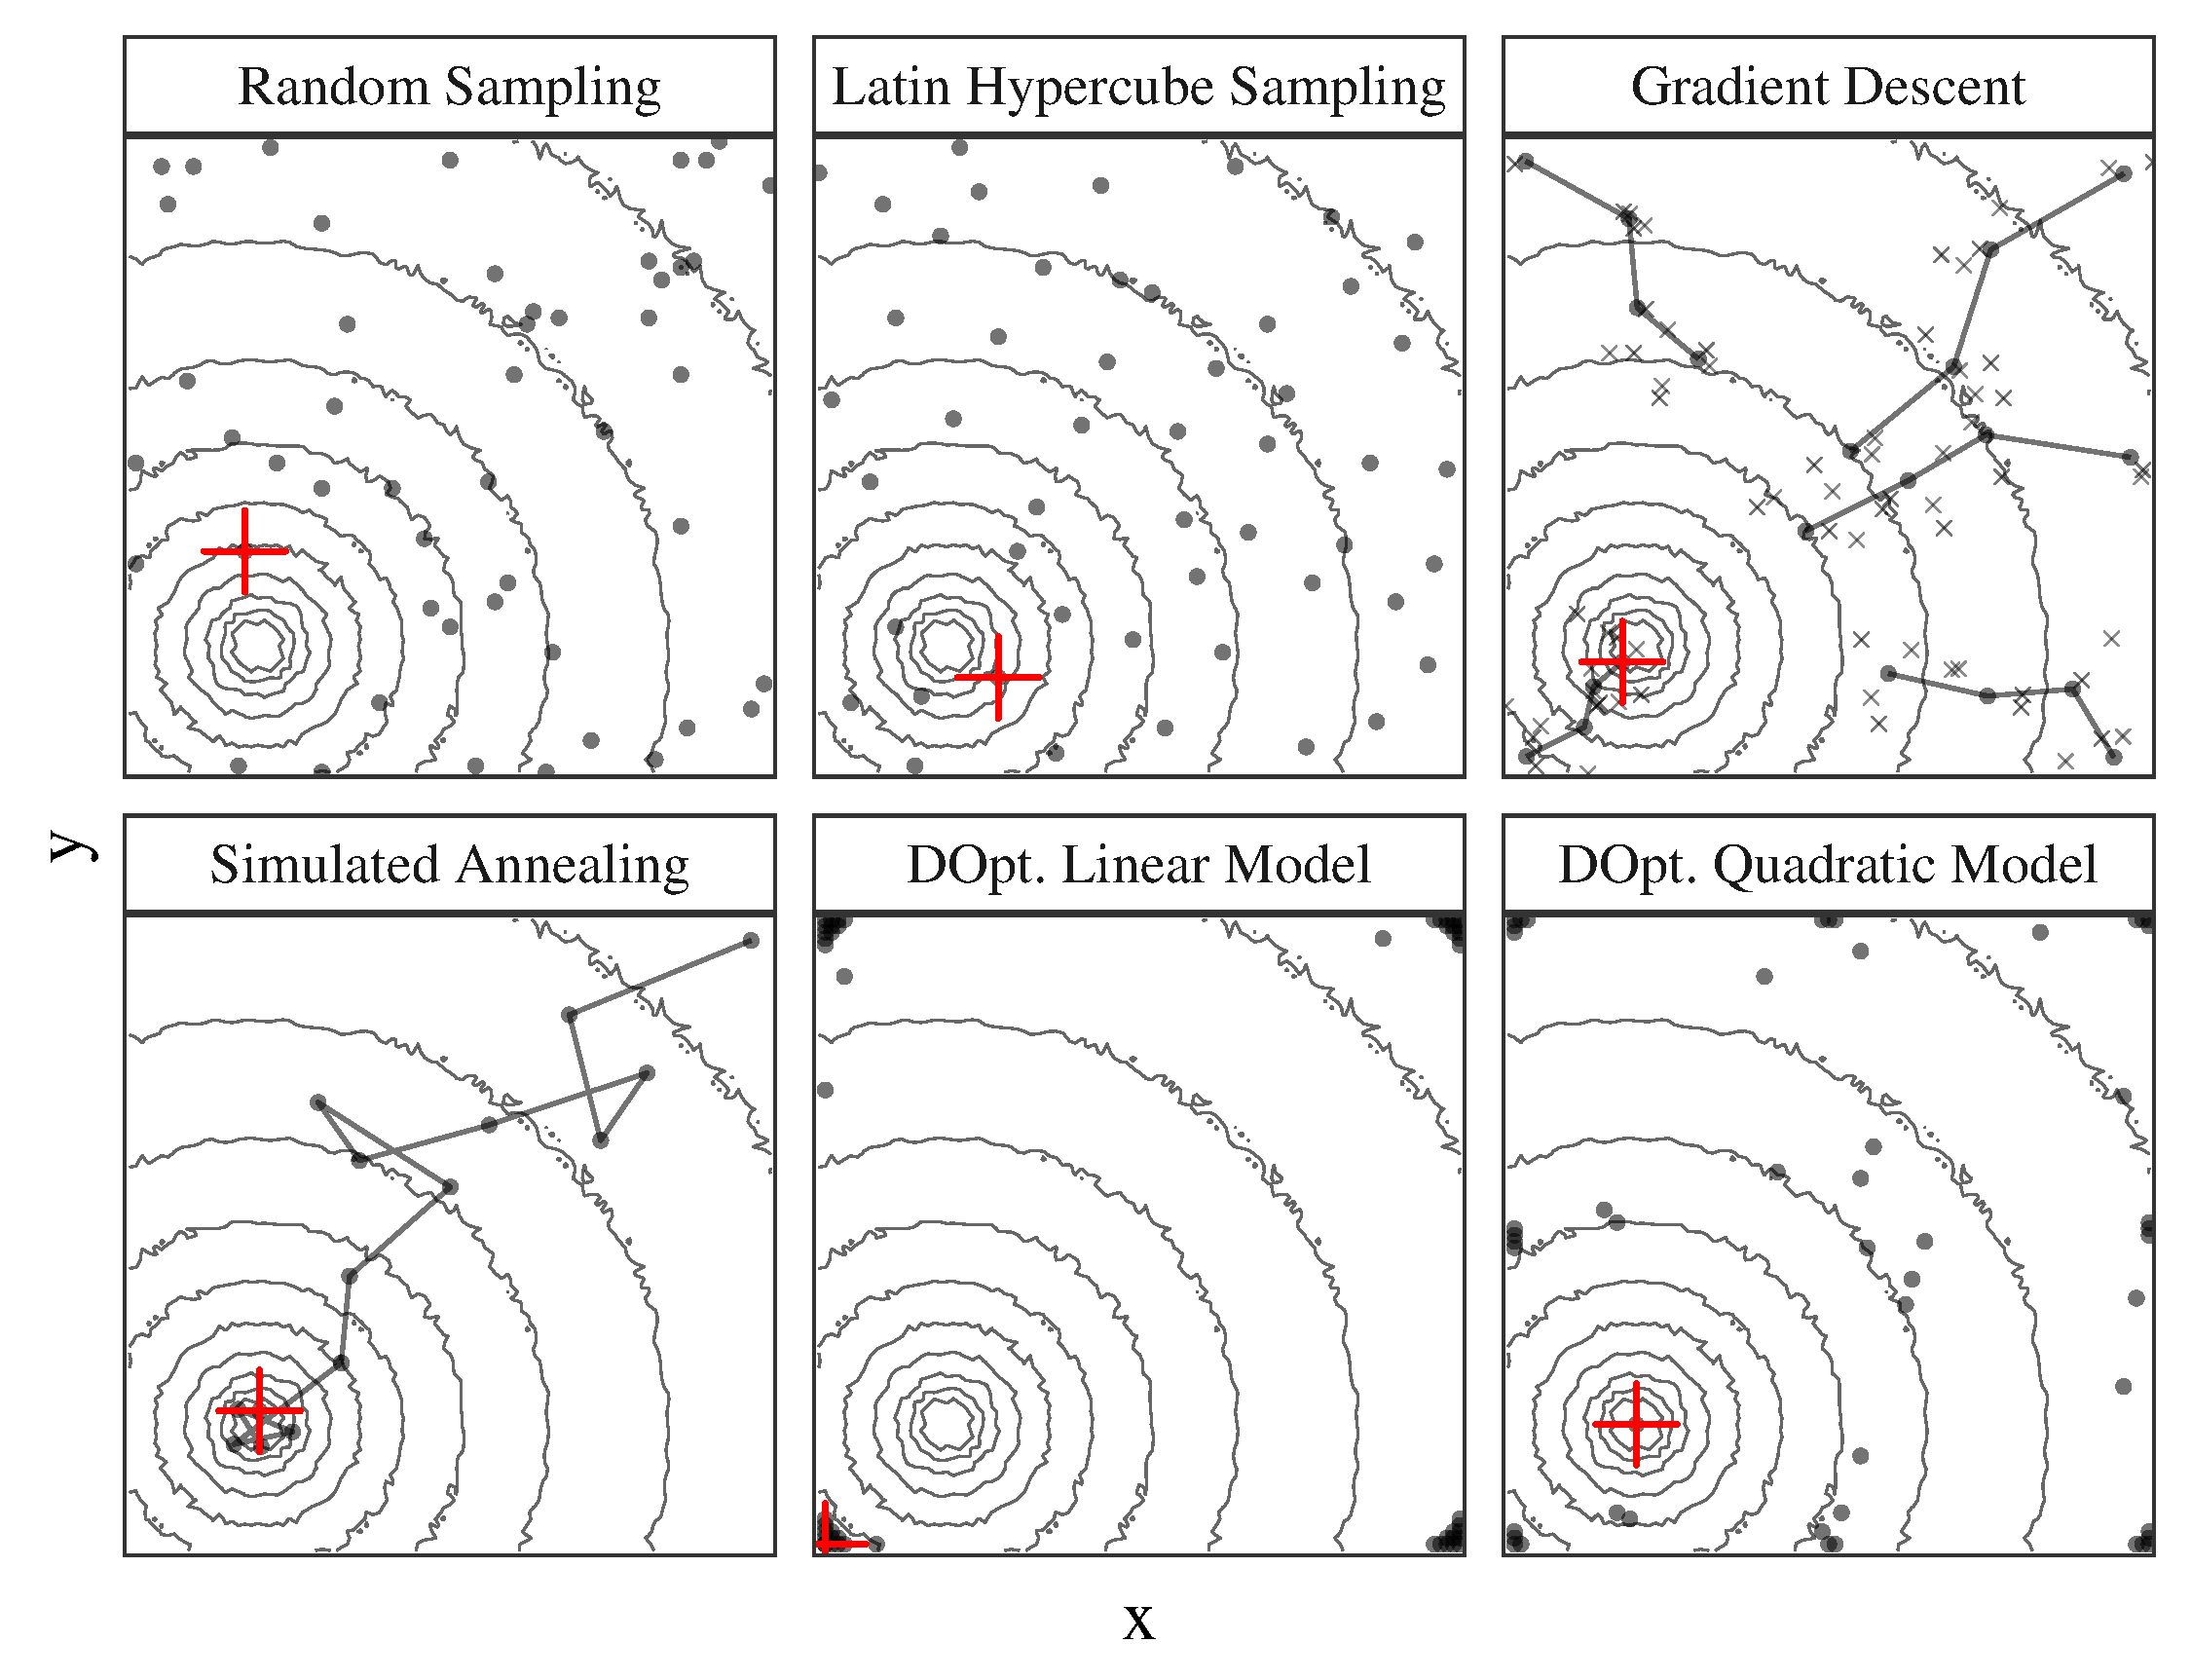
\includegraphics[width=.72\textwidth]{../../../img/sampling_comparison.pdf}
\end{center}
\end{center}
\end{frame}
\section{Case Study: HLS for FPGAs}
\label{sec:orgead503d}
\begin{frame}[label={sec:orgd26ffeb}]{An Example Using Meta-Heuristics: HLS for FPGAs}
\begin{columns}
\begin{column}{0.4\columnwidth}
\begin{block}{Autotuning HLS for FPGAs}
\begin{itemize}
\item CHStone benchmark
\item 141 factors, most with multiple levels
\item \alert{\(10^{128}\)} combinations
\item \alert{1\textasciitilde{}10min} to measure
\item \alert{Multiple objectives}
\item Search with meta-heuristics:
\begin{itemize}
\item Unstructured data hinders analysis
\end{itemize}
\end{itemize}
\end{block}
\end{column}
\begin{column}{0.6\columnwidth}
\begin{block}{Coverage of the Design Space}
\begin{center}
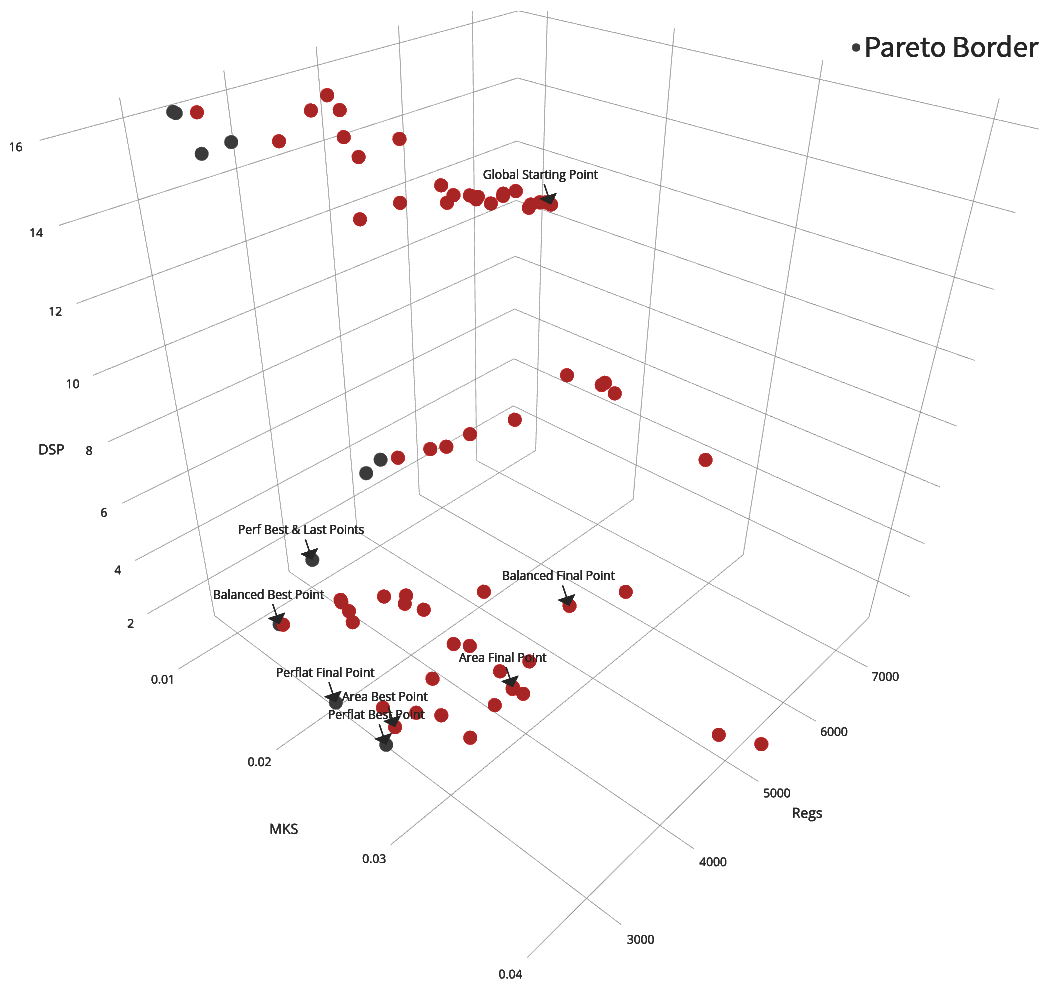
\includegraphics[width=.85\columnwidth]{../../../img/fpga_space.png}
\end{center}
\end{block}
\end{column}
\end{columns}
\end{frame}
\begin{frame}[label={sec:org41d897b}]{Results: Targeting Performance}
\begin{columns}
\begin{column}{0.2\columnwidth}
\begin{block}{Metric Weights}
\begin{table}[htpb]
  \scriptsize
  \centering
  \begin{tabular}{@{}lcccc@{}}
    \toprule
    Metric & \textit{Performance} \\ \midrule
    \textit{LUT} & \cellcolor[HTML]{DD9583} Low \\
    \textit{Registers} & \cellcolor[HTML]{E3DBB3} Medium \\
    \textit{BRAMs} & \cellcolor[HTML]{DD9583} Low \\
    \textit{DSPs} & \cellcolor[HTML]{DD9583} Low \\
    \textit{FMax} & \cellcolor[HTML]{9B94B6} High \\
    \textit{Cycles} & \cellcolor[HTML]{DD9583} Low \\ \bottomrule
  \end{tabular}
\end{table}
\end{block}
\end{column}
\begin{column}{0.8\columnwidth}
\begin{block}{Improvements after 1.5h of Autotuning}
\begin{center}
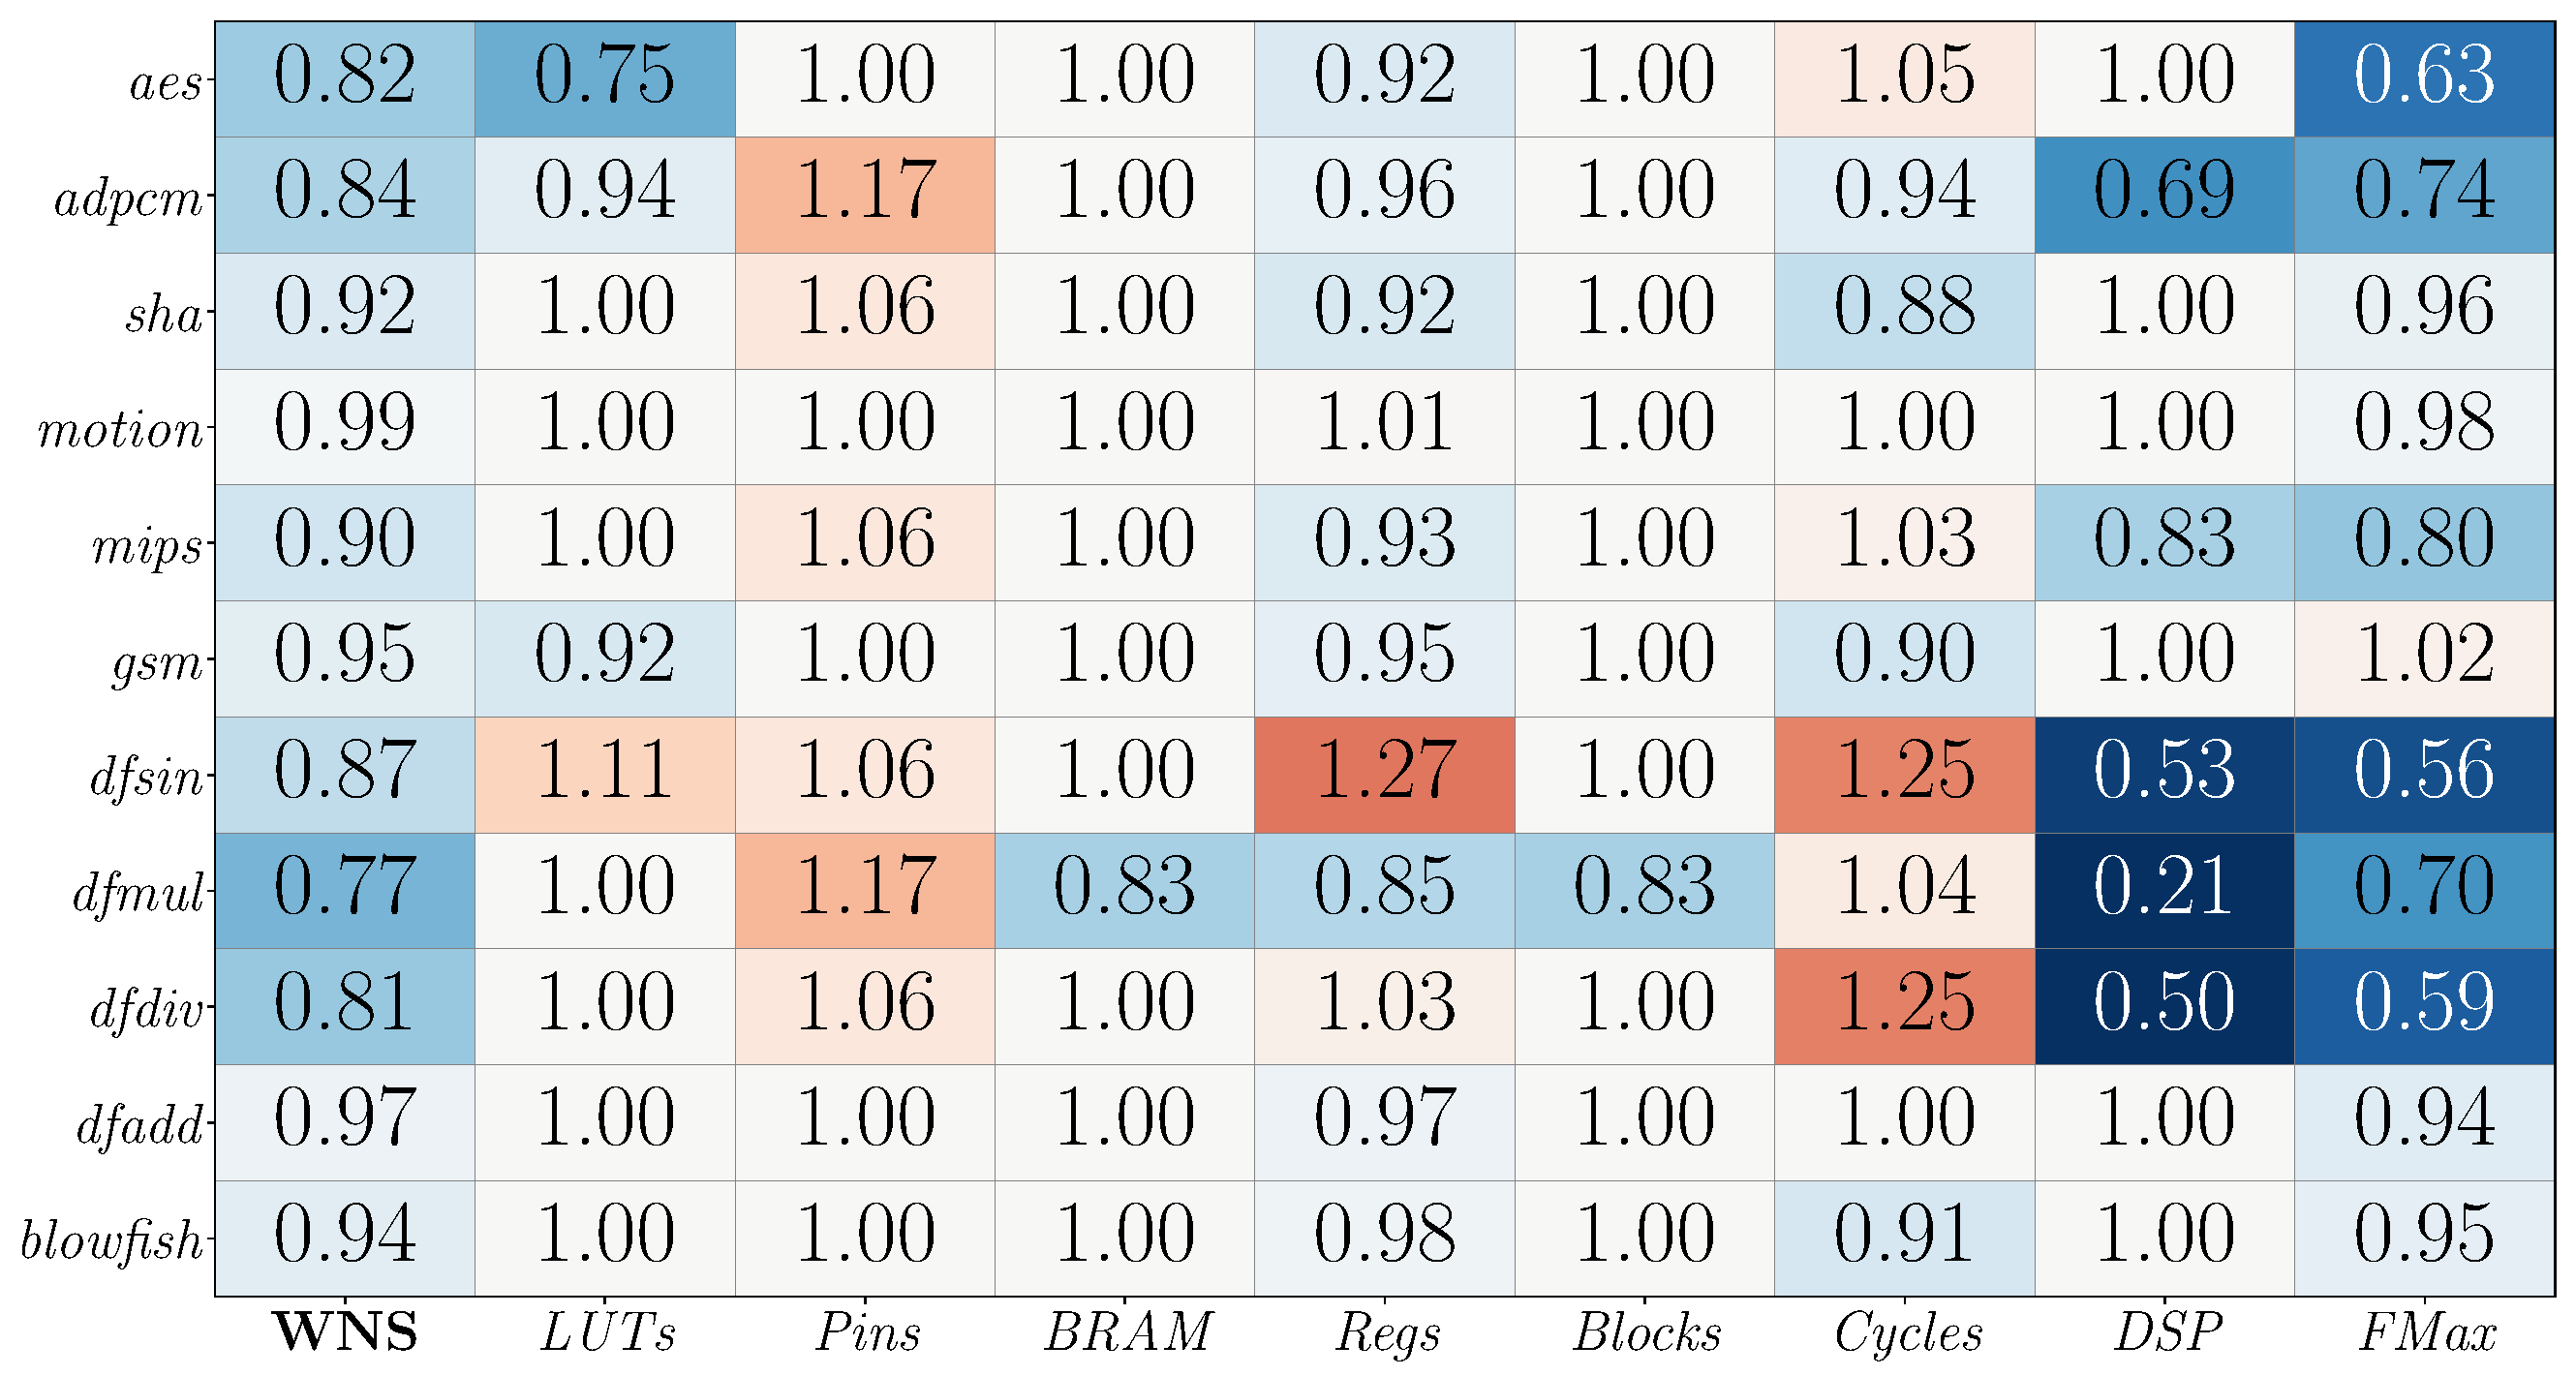
\includegraphics[width=.9\linewidth]{../../../img/heatmap_default_stratixV_perf-eps-converted-to.pdf}
\end{center}

\begin{center}
\scriptsize{Autotuning high-level synthesis for \\ FPGAs using OpenTuner and LegUp (ReConFig 2017)}
\end{center}
\end{block}
\end{column}
\end{columns}
\end{frame}

\section{A Transparent and Parsimonious ED Approach to Autotuning}
\label{sec:org6a976d1}
\begin{frame}[label={sec:org80e37fc}]{A Experimental Design Approach to Autotuning}
\begin{center}
\begin{center}
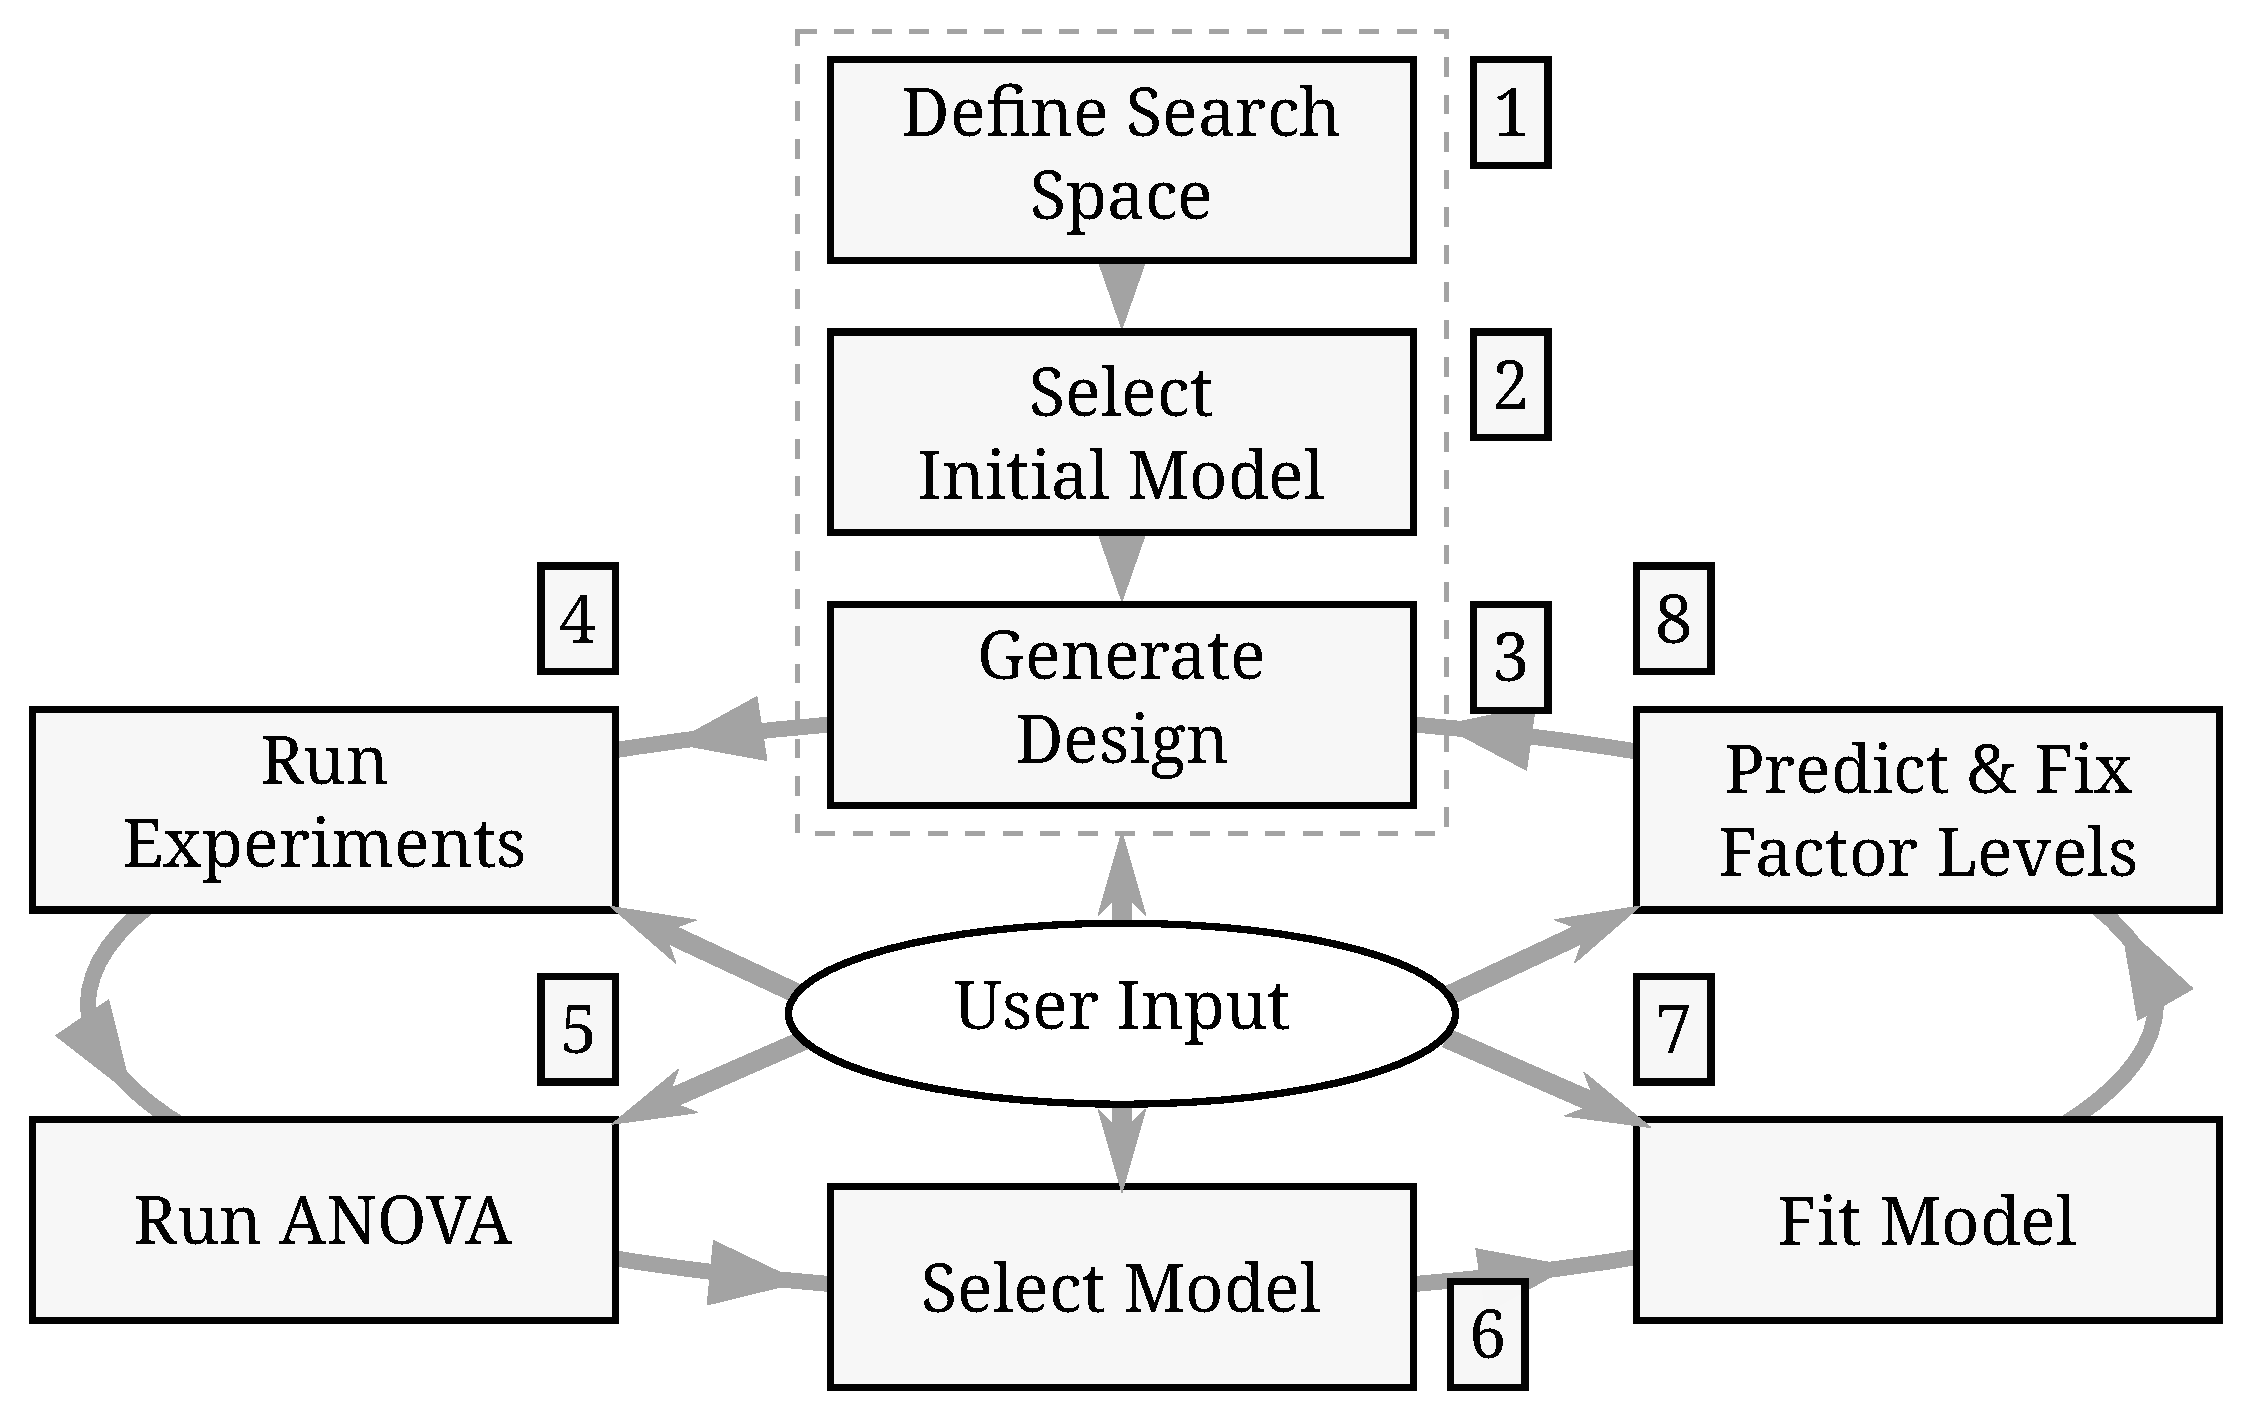
\includegraphics[width=.74\linewidth]{../../../img/doe_anova_strategy.pdf}
\end{center}

\vspace{-.2cm}
\end{center}

\begin{center}
\scriptsize{Autotuning under Tight Budget Constraints: \\ A Transparent Design of Experiments Approach (CCGRID 2019)}
\end{center}
\end{frame}
\section{Results on a GPU Laplacian Kernel}
\label{sec:org59e25ad}
\begin{frame}[label={sec:org90caa52}]{GPU Laplacian Kernel: A Motivating Example}
\begin{columns}
\begin{column}{0.5\columnwidth}
\begin{block}{Search Problem}
\begin{itemize}
\item Relatively small valid search space
\item Completely evaluated
\item Global optimum is \alert{known}
\item Budget of \alert{125 points}
\end{itemize}
\end{block}
\end{column}

\begin{column}{0.5\columnwidth}
\begin{block}{Initial Model}
\footnotesize
\begin{align*}
cost = & \; y\_component\_number + 1 / y\_component\_number \; + \\
& \; vector\_length + lws\_y + 1 / lws\_y \; + \\
& \; load\_overlap + temporary\_size \; + \\
& \; elements\_number + 1 / elements\_number \; + \\
& \; threads\_number + 1 / threads\_number
\end{align*}
\normalsize
\end{block}
\end{column}
\end{columns}

\vspace{-.3cm}

\uncover<2>{
\begin{center}
  \colorbox{Highlight}{\parbox[c]{0.72\textwidth}{\centering We were  always close to
        the \alert{optimum} and used \alert{half of the budget}}}
\end{center}
}

\vspace{-.3cm}

\begin{center}
\begin{center}
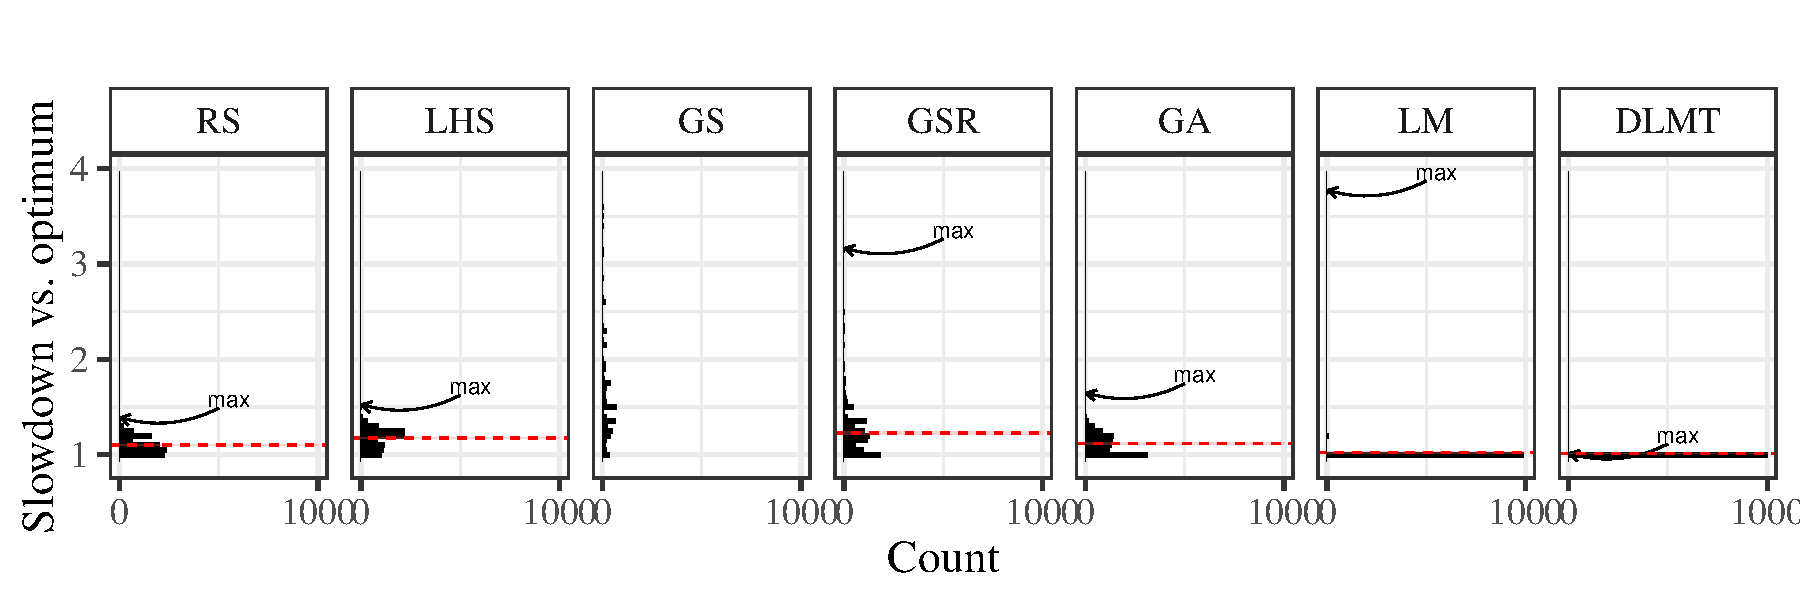
\includegraphics[width=.88\columnwidth]{../../../img/comparison_histogram.pdf}
\end{center}
\end{center}
\end{frame}
\section{Results on the SPAPT Benchmark}
\label{sec:org805f712}
\begin{frame}[label={sec:org92aa806},fragile]{SPAPT: Search Problems in Automatic Performance Tuning}
 \begin{columns}
\begin{column}{0.41\columnwidth}
\begin{block}{Search Problem}
\begin{itemize}
\item Orio: source code transformation
\item Baseline: \texttt{gcc -O3}, no transformations
\item Random sampling (\alert{RS}) vs. D-Optimal approach (\alert{DLMT})
\item 10 repetitions: measure \alert{speedup} and \alert{time-to-solution}
\item Out of 16 kernels:
\begin{itemize}
\item 3 with no impact
\item 6 with similar performance gains
\item \colorbox{Highlight}{7 with \alert{gains found faster}}
\end{itemize}
\end{itemize}
\end{block}
\end{column}
\begin{column}{0.59\columnwidth}
\begin{block}{Search Space}
\vspace{-0.4cm}

\begin{center}
\begin{table}[t]
\label{tab:org238b383}
\centering
\scriptsize
\begin{tabular}{llll}
\toprule
Kernel & Operation & Factors & Size\\
\midrule
\texttt{atax} & Matrix transp. \& vector mult. & 18 & \(2.6 \times 10^{16}\)\\
\texttt{dgemv3} & Scalar, vector \& matrix mult. & 49 & \(3.8 \times 10^{36}\)\\
\texttt{gemver} & Vector mult. \& matrix add. & 24 & \(2.6 \times 10^{22}\)\\
\texttt{gesummv} & Scalar, vector, \& matrix mult. & 11 & \(5.3 \times 10^{9}\)\\
\texttt{hessian} & Hessian computation & 9 & \(3.7 \times 10^{7}\)\\
\texttt{mm} & Matrix multiplication & 13 & \(1.2 \times 10^{12}\)\\
\texttt{mvt} & Matrix vector product \& transp. & 12 & \(1.1 \times 10^{9}\)\\
\texttt{tensor} & Tensor matrix mult. & 20 & \(1.2 \times 10^{19}\)\\
\texttt{trmm} & Triangular matrix operations & 25 & \(3.7 \times 10^{23}\)\\
\texttt{bicg} & Subkernel of BiCGStab & 13 & \(3.2 \times 10^{11}\)\\
\texttt{lu} & LU decomposition & 14 & \(9.6 \times 10^{12}\)\\
\texttt{adi} & Matrix sub., mult., \& div. & 20 & \(6.0 \times 10^{15}\)\\
\texttt{jacobi} & 1-D Jacobi computation & 11 & \(5.3 \times 10^{9}\)\\
\texttt{seidel} & Matrix factorization & 15 & \(1.3 \times 10^{14}\)\\
\texttt{stencil3d} & 3-D stencil computation & 29 & \(9.7 \times 10^{27}\)\\
\texttt{correlation} & Correlation computation & 21 & \(4.5 \times 10^{17}\)\\
\bottomrule
\end{tabular}
\end{table}

\scriptsize{Balaprakash P, Wild SM, Norris B. SPAPT: Search problems in automatic performance tuning. Procedia Comp. Sci. 2012 Jan 1;9:1959-68.}
\end{center}
\end{block}
\end{column}
\end{columns}
\end{frame}

\begin{frame}[label={sec:org9be8c66}]{SPAPT: Search Problems in Automatic Performance Tuning}
\begin{center}
\begin{center}
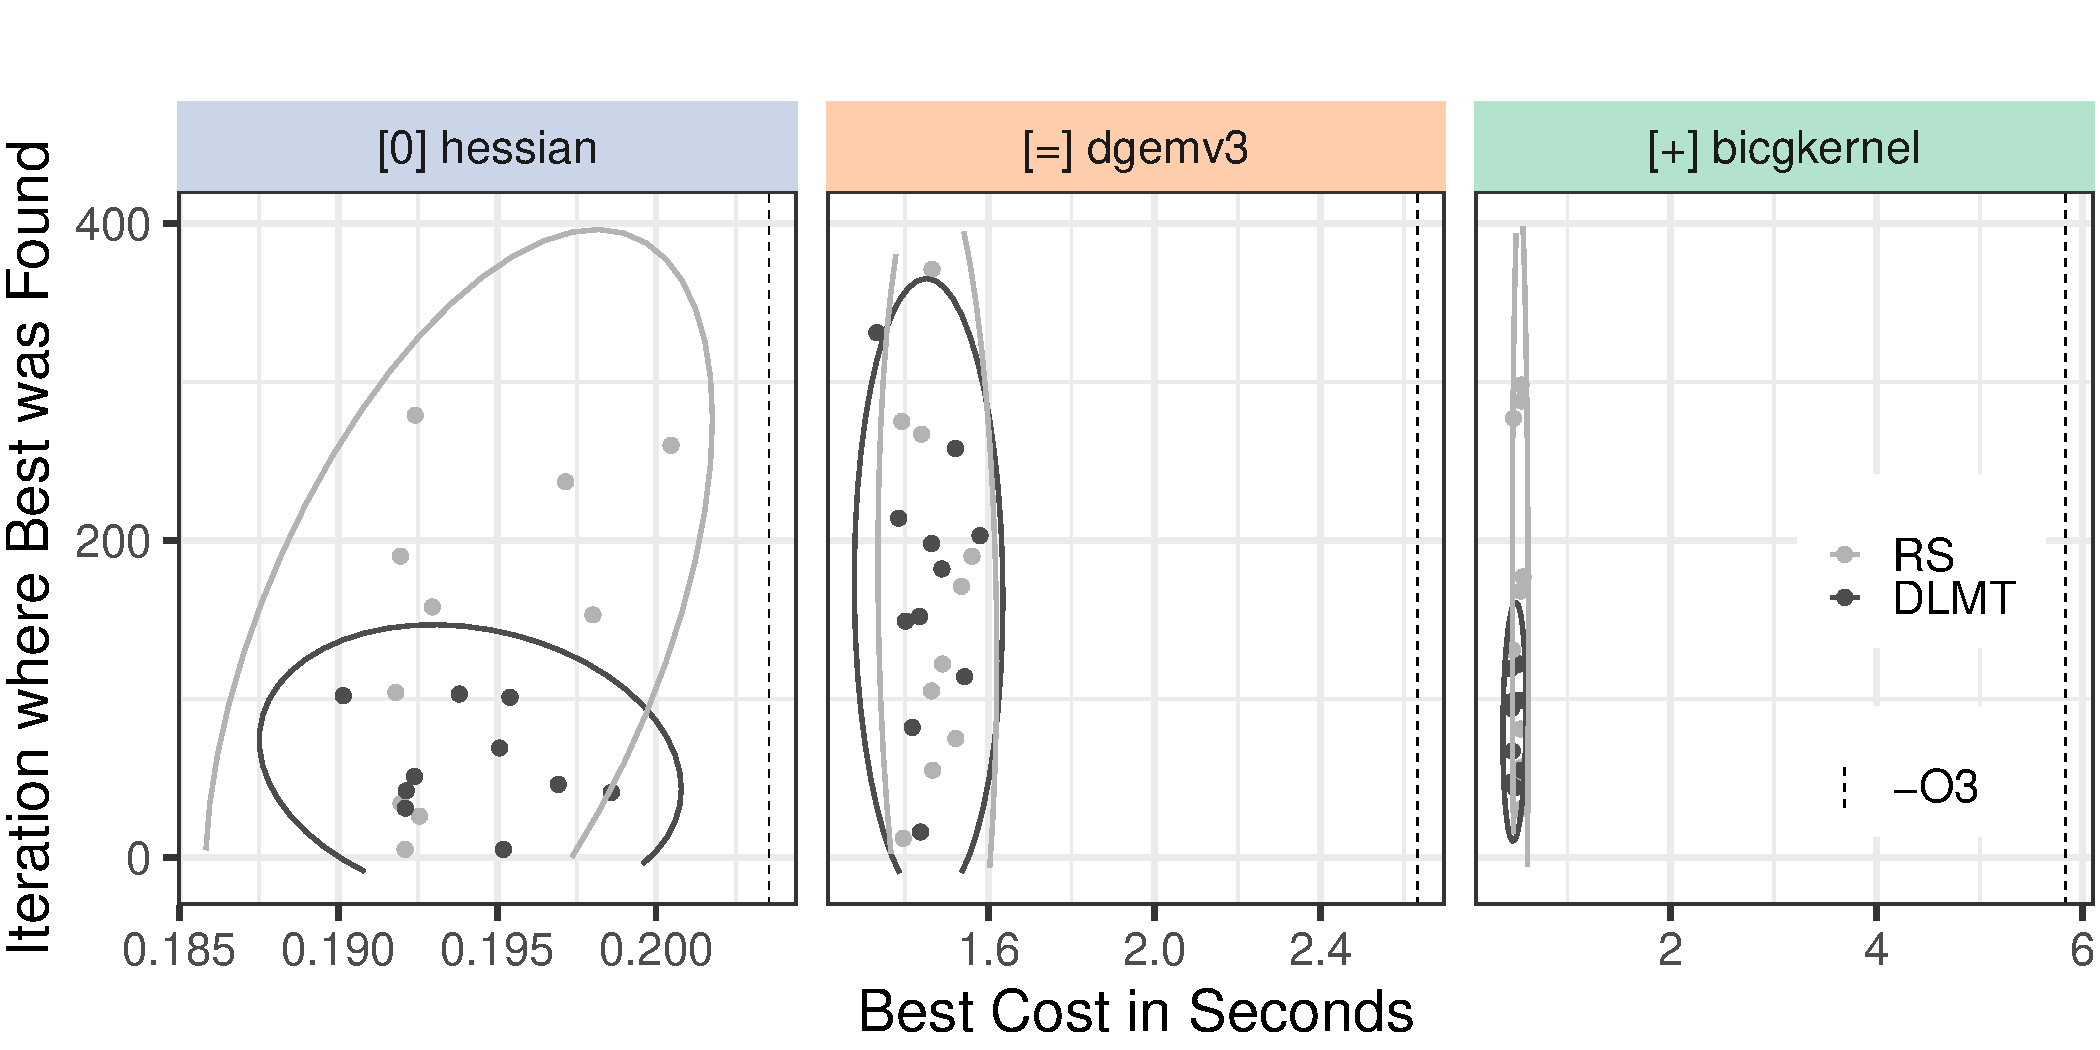
\includegraphics[width=\linewidth]{../../../img/iteration_best_comparison.pdf}
\end{center}
\end{center}
\end{frame}
\begin{frame}[label={sec:org54ebfeb}]{SPAPT: Search Problems in Automatic Performance Tuning}
\begin{center}
\begin{center}
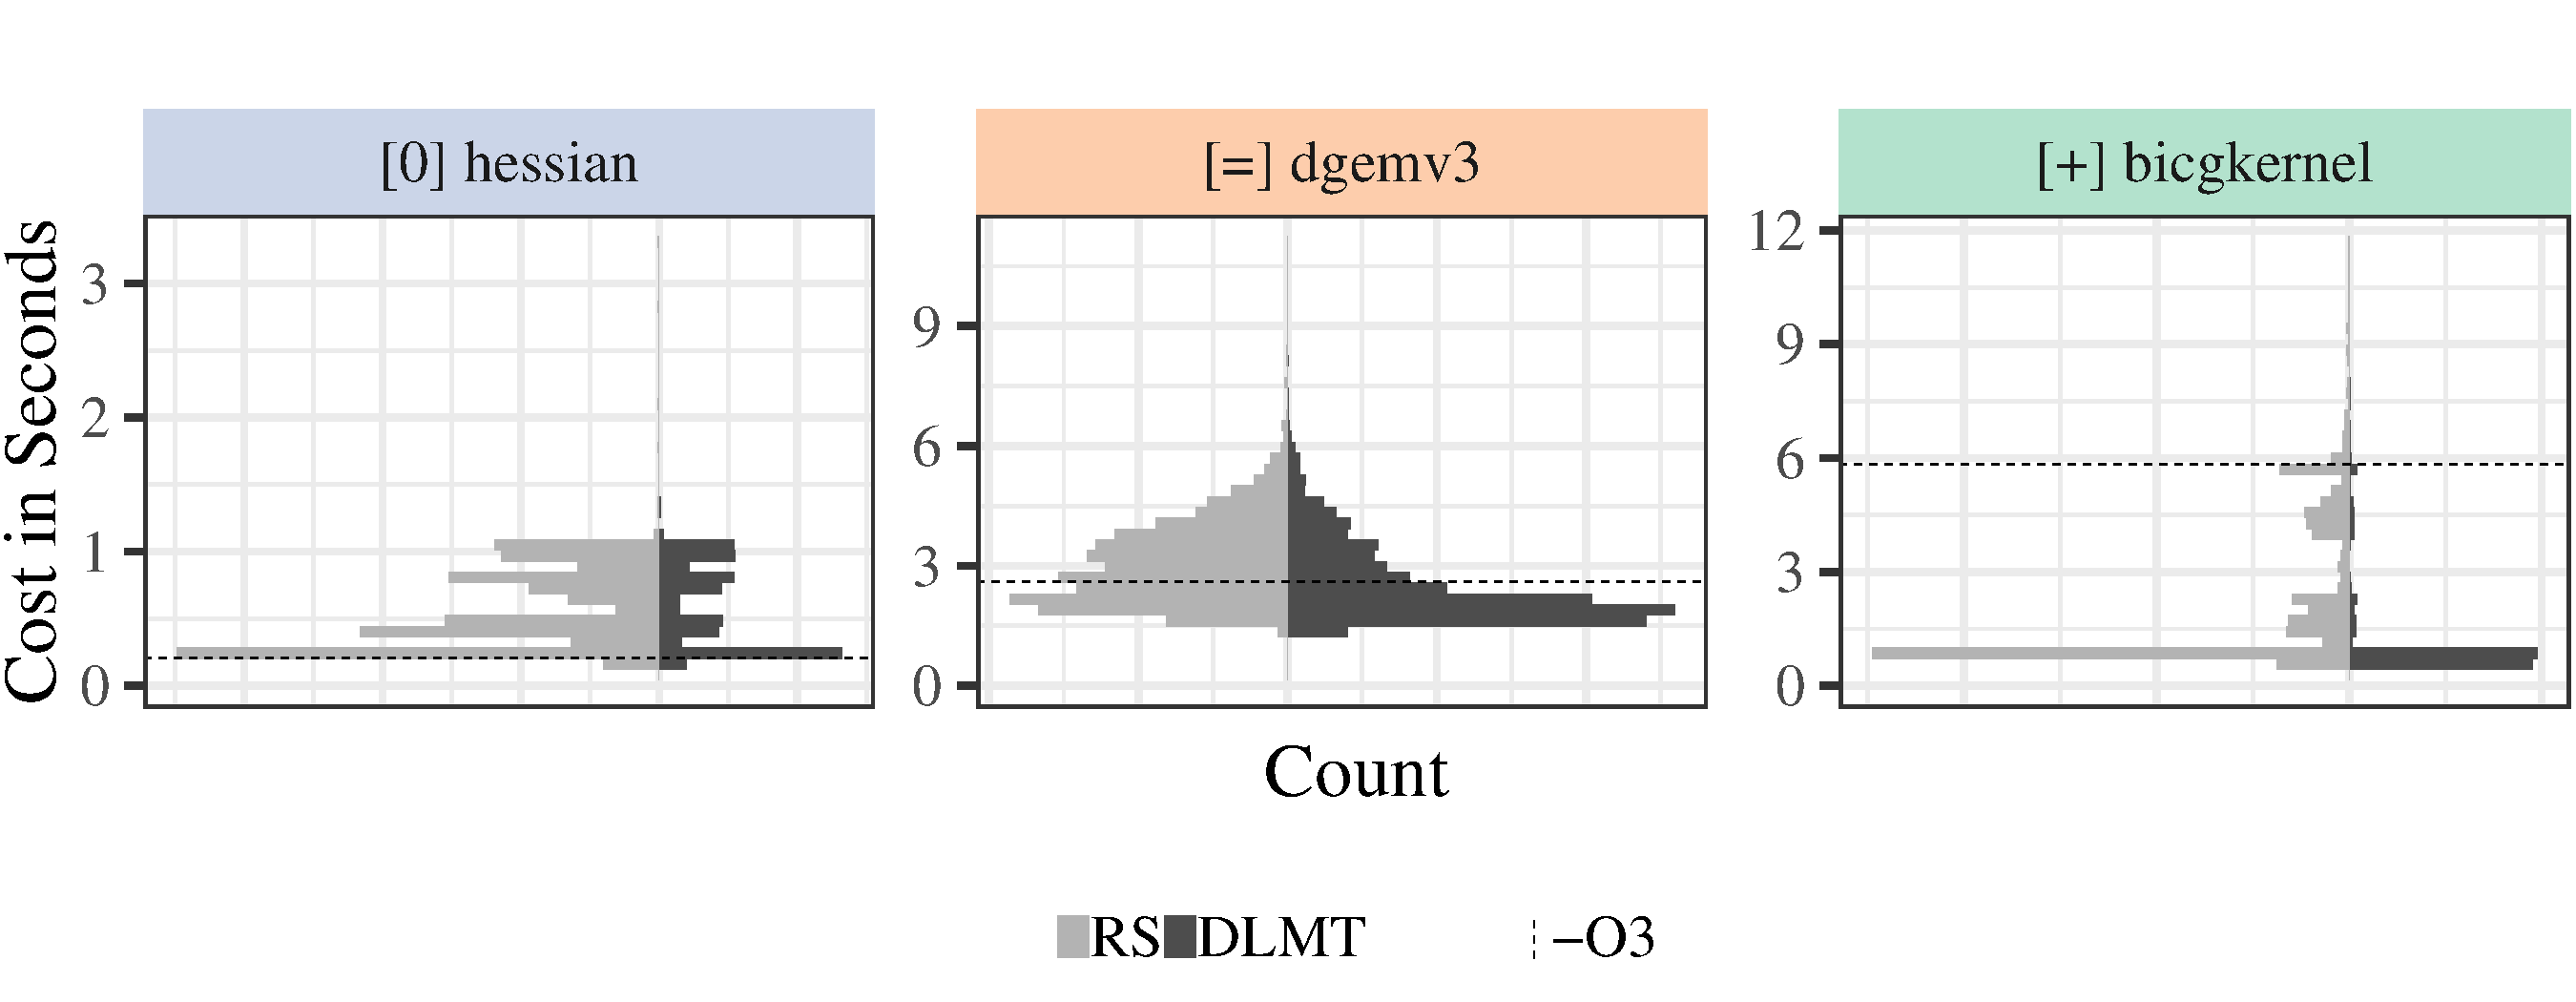
\includegraphics[width=\linewidth]{../../../img/split_histograms.pdf}
\end{center}
\end{center}
\end{frame}
\begin{frame}[label={sec:orga68a80a},fragile]{SPAPT: Optimizing \texttt{bicgkernel}}
 \begin{center}
\begin{center}
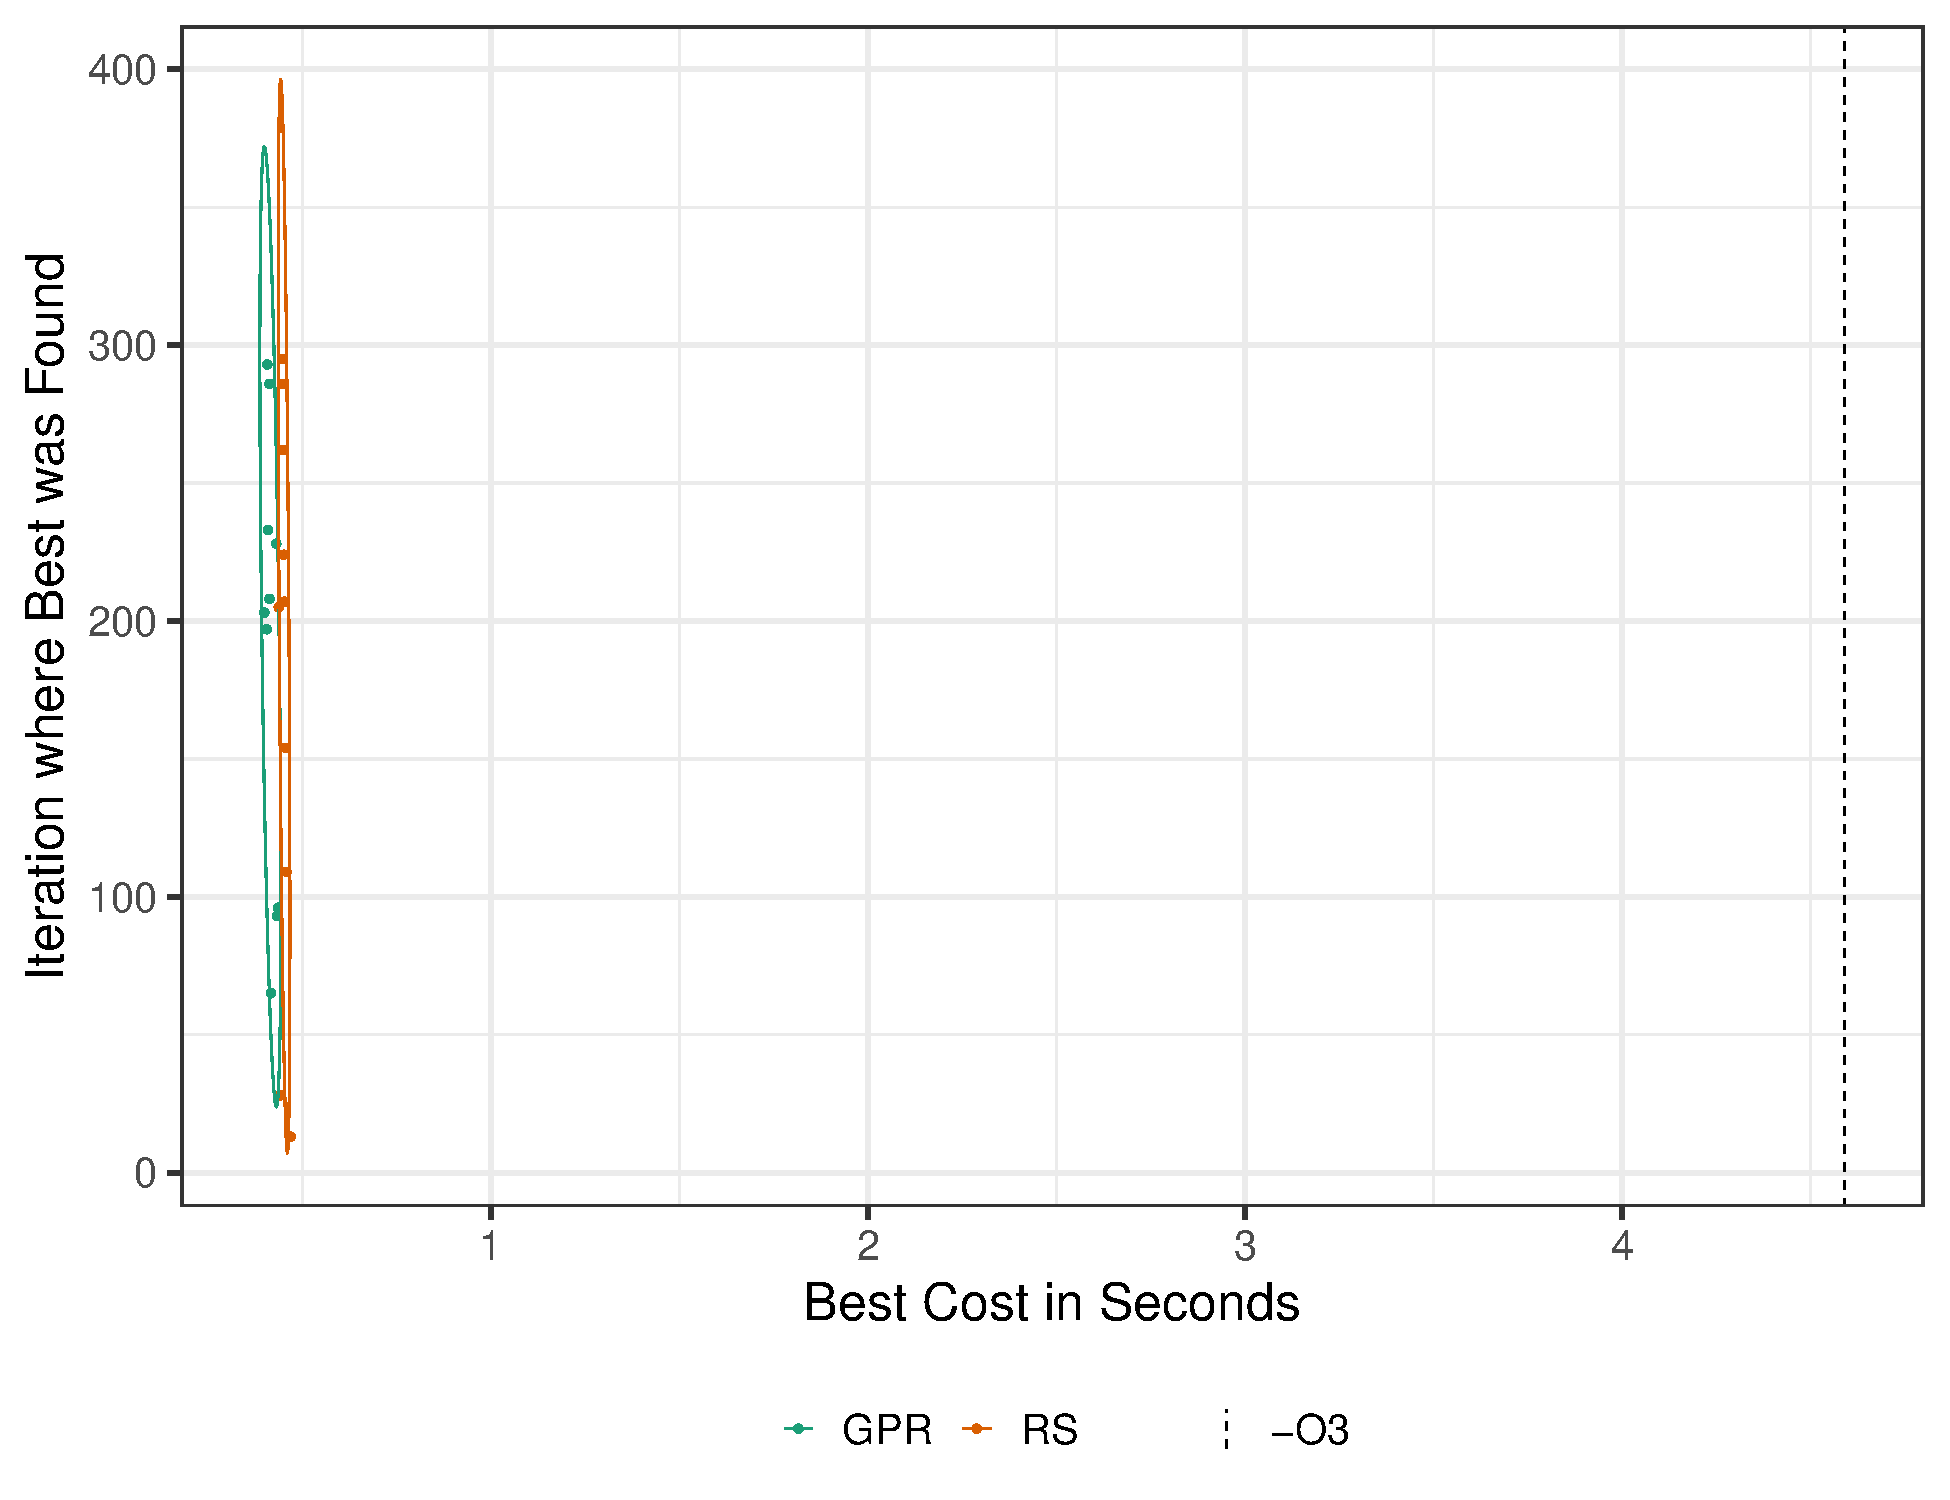
\includegraphics[width=.7\columnwidth]{../../../img/updated_bicgkernel_I.pdf}
\end{center}
\end{center}
\end{frame}
\begin{frame}[label={sec:org88dae01},fragile]{SPAPT: Optimizing \texttt{bicgkernel}}
 \begin{center}
\begin{center}
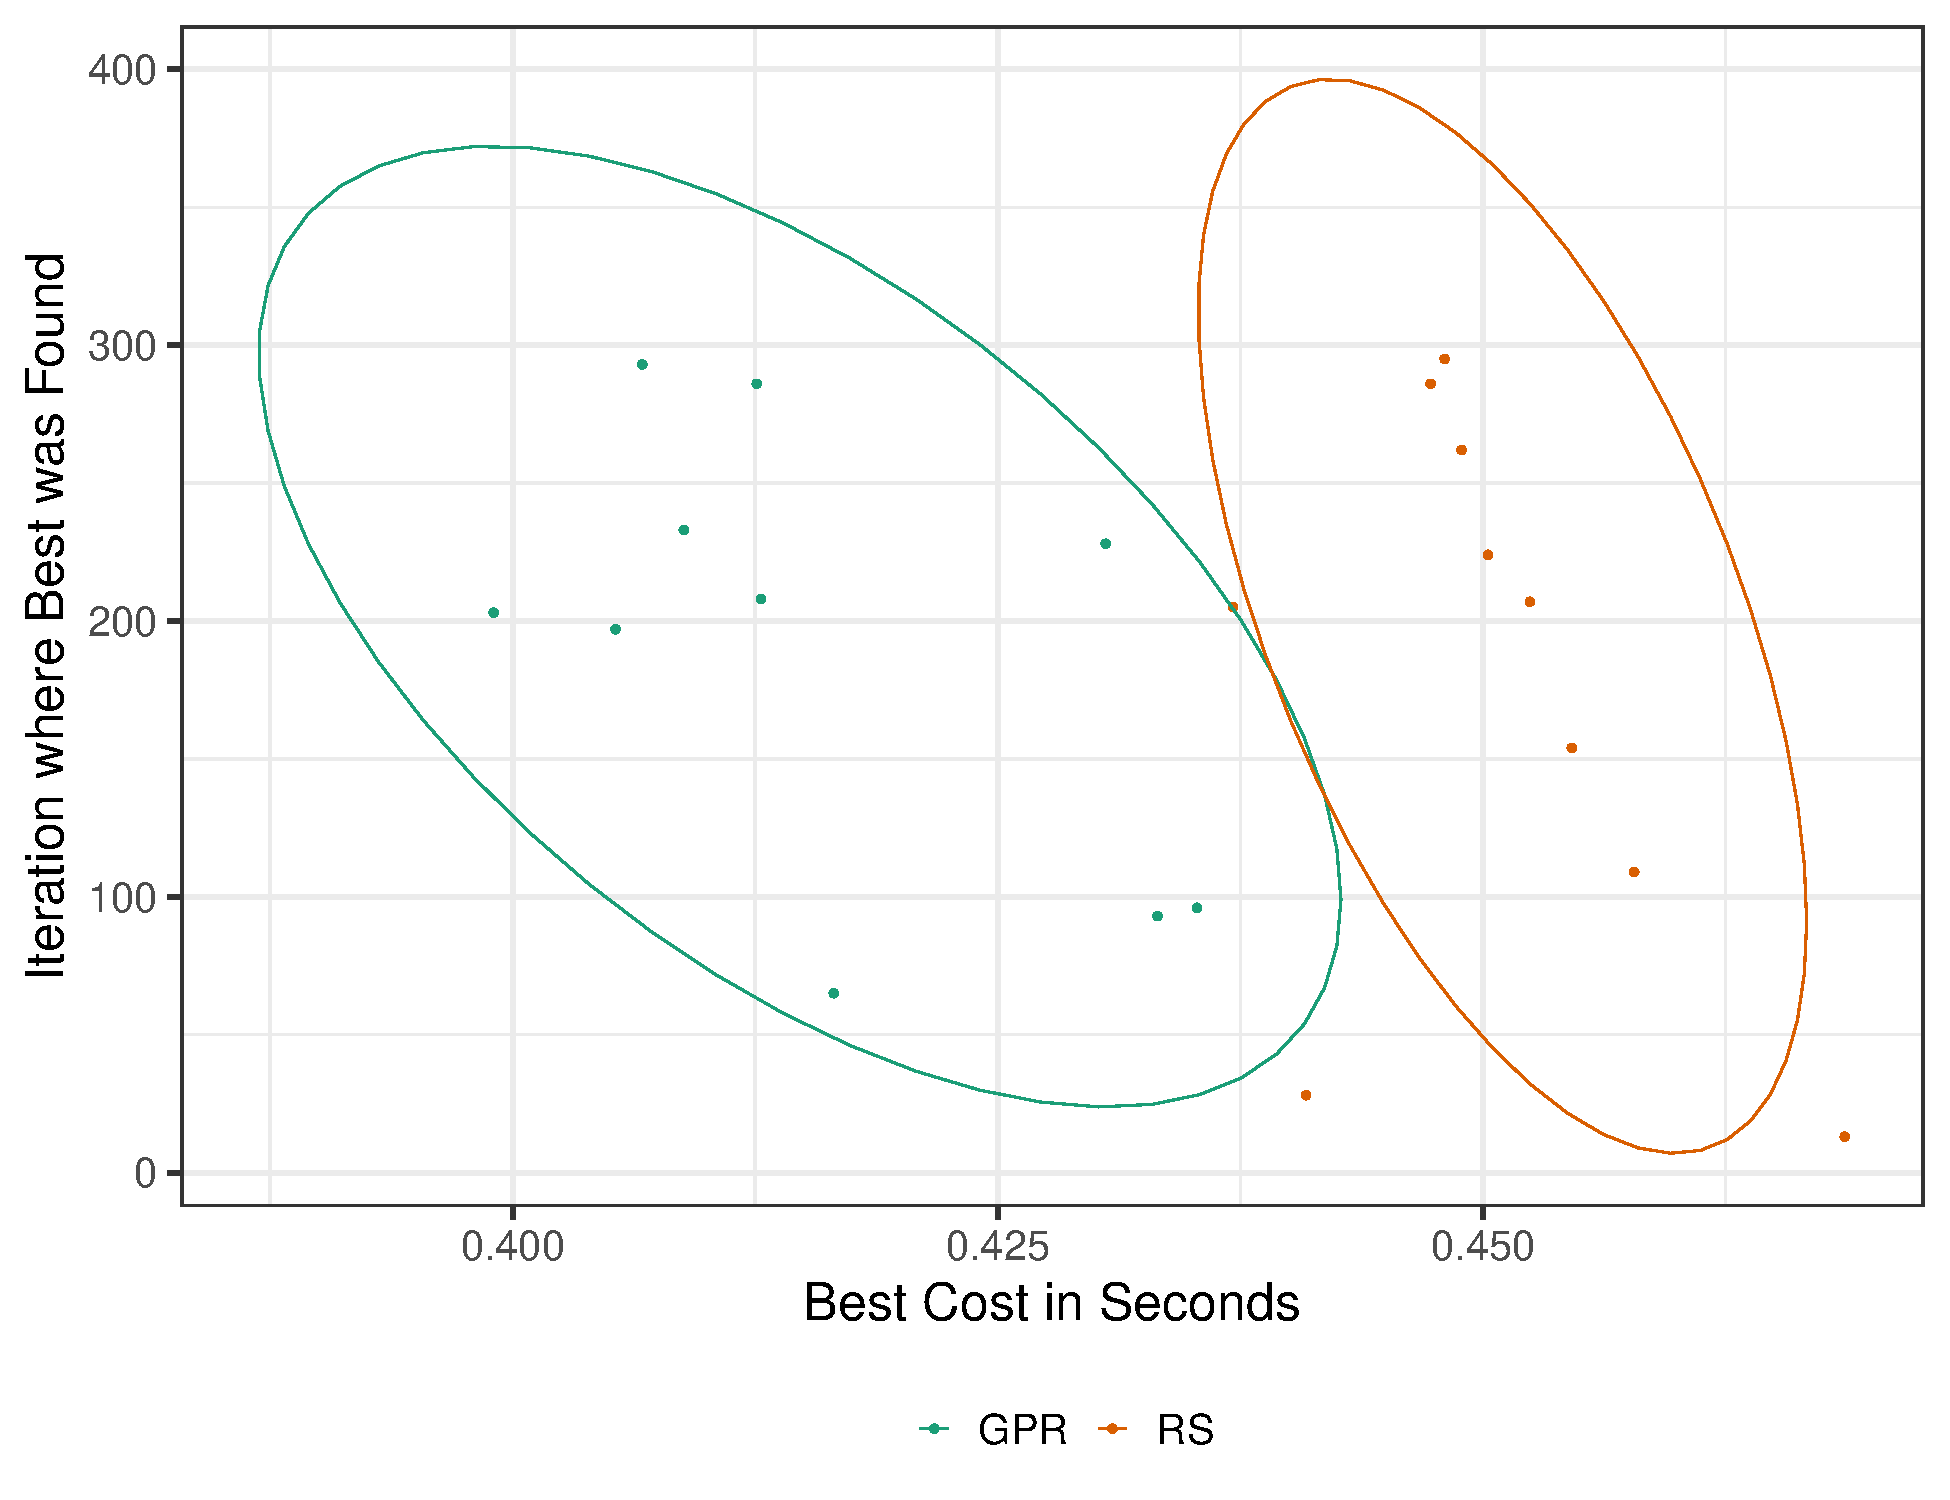
\includegraphics[width=.7\columnwidth]{../../../img/updated_bicgkernel.pdf}
\end{center}
\end{center}
\end{frame}
\section{Next Steps}
\label{sec:org90dc29b}
\begin{frame}[label={sec:org30ac61a}]{Next Steps: Two months at Hewlett Packard Labs}
\begin{block}{Apply Experimental Design methods on:}
\begin{itemize}
\item Design space exploration for \alert{quantization} on DNN layers
\item Neural Architecture Search (\alert{NAS}) on CPUs and GPUs
\end{itemize}
\end{block}
\end{frame}
\begin{frame}[label={sec:orgae31bb9}]{Quantization on DNN Layers}
\begin{center}
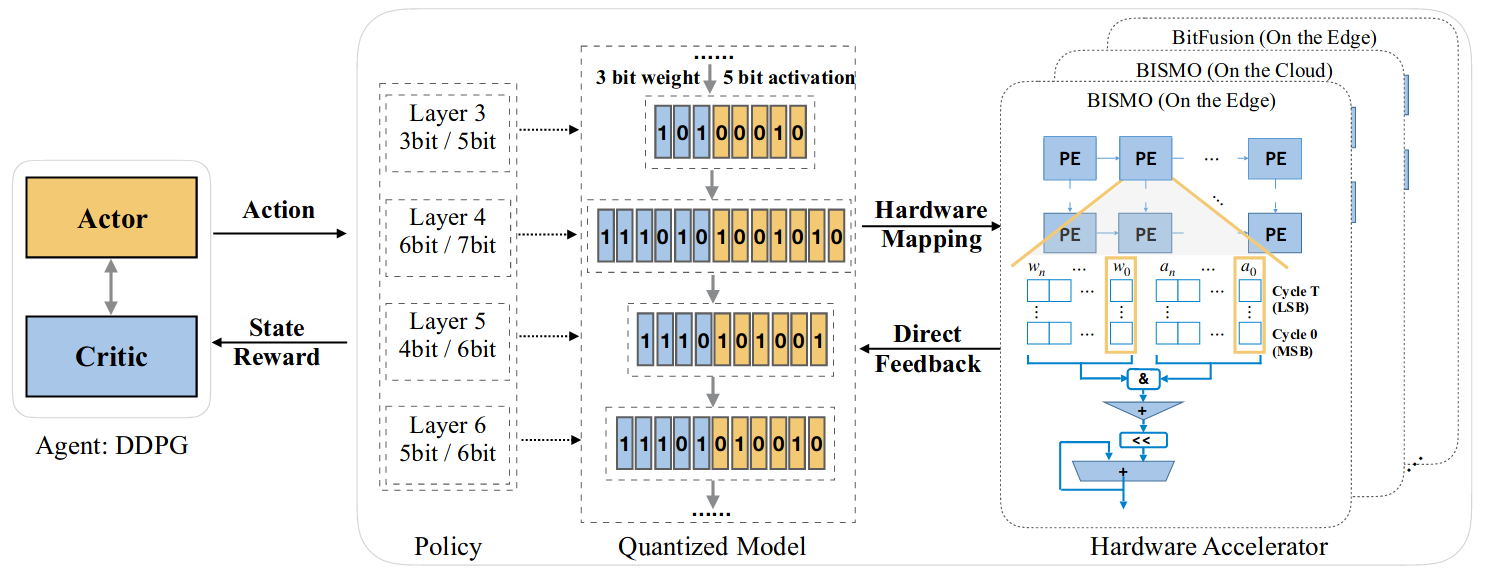
\includegraphics[width=\columnwidth]{../../../img/haq_quantization.png}
\end{center}

\begin{center}
\scriptsize{HAQ: Hardware-Aware Automated Quantization with Mixed Precision (CV 2018)}
\end{center}
\end{frame}

\begin{frame}[label={sec:orgb52ab38}]{Quantization on DNN Layers}
\begin{center}
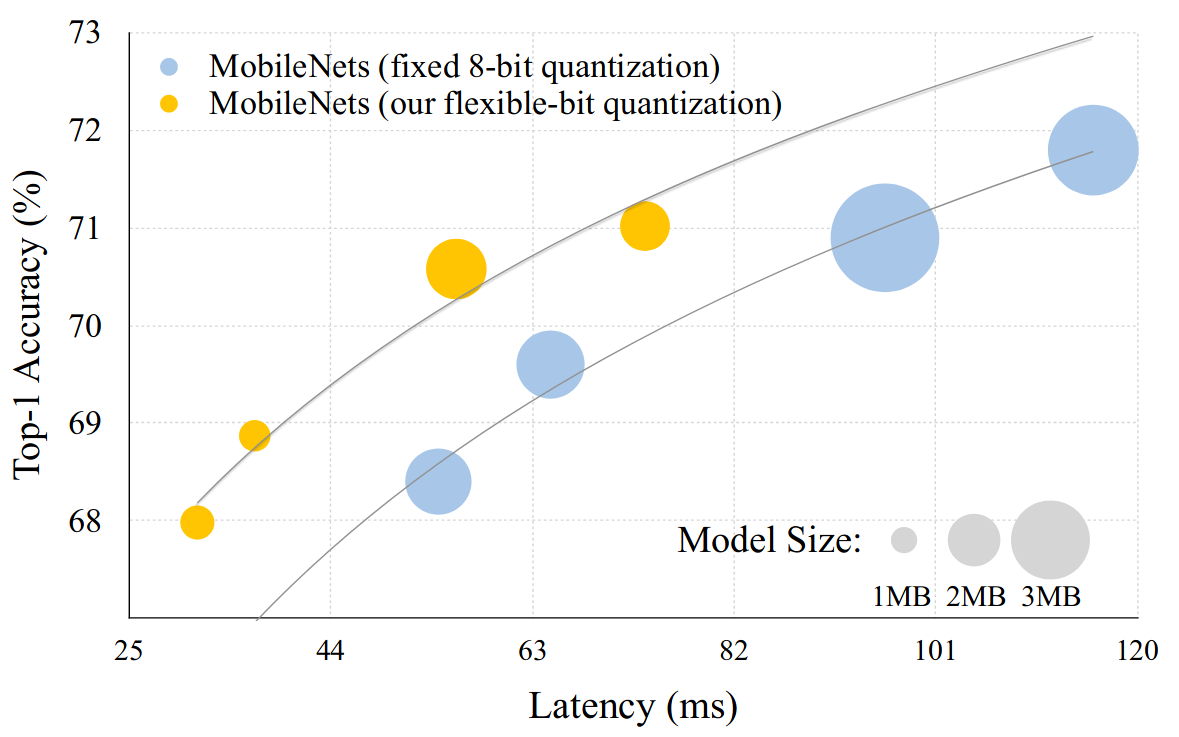
\includegraphics[width=.7\columnwidth]{../../../img/haq_quantization_II.png}
\end{center}

\begin{center}
\scriptsize{HAQ: Hardware-Aware Automated Quantization with Mixed Precision (CV 2018)}
\end{center}
\end{frame}

\begin{frame}[label={sec:org71dc6e7}]{Neural Architecture Search}
\begin{center}
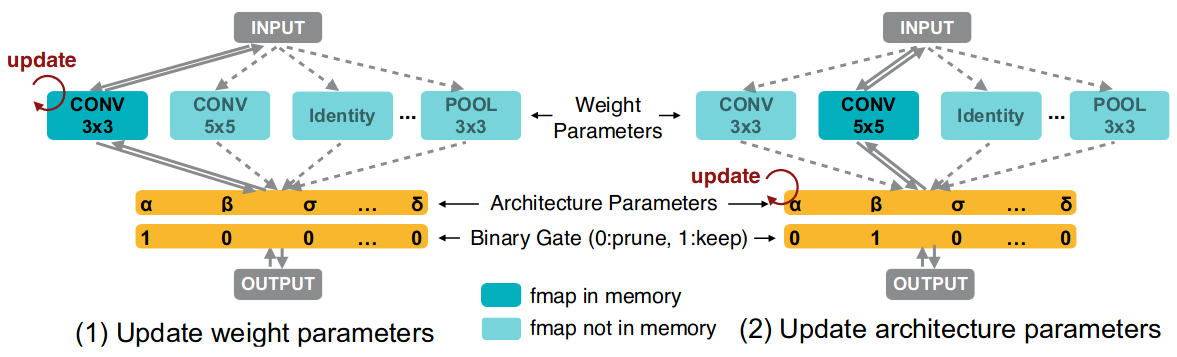
\includegraphics[width=.9\columnwidth]{../../../img/proxylessnas_III.png}
\end{center}

\begin{center}
\scriptsize{ProxylessNAS: Direct Neural Architecture Search on Target Task and Hardware (ICLR 2019)}
\end{center}
\end{frame}

\begin{frame}[label={sec:orgc968031}]{Neural Architecture Search}
\begin{center}
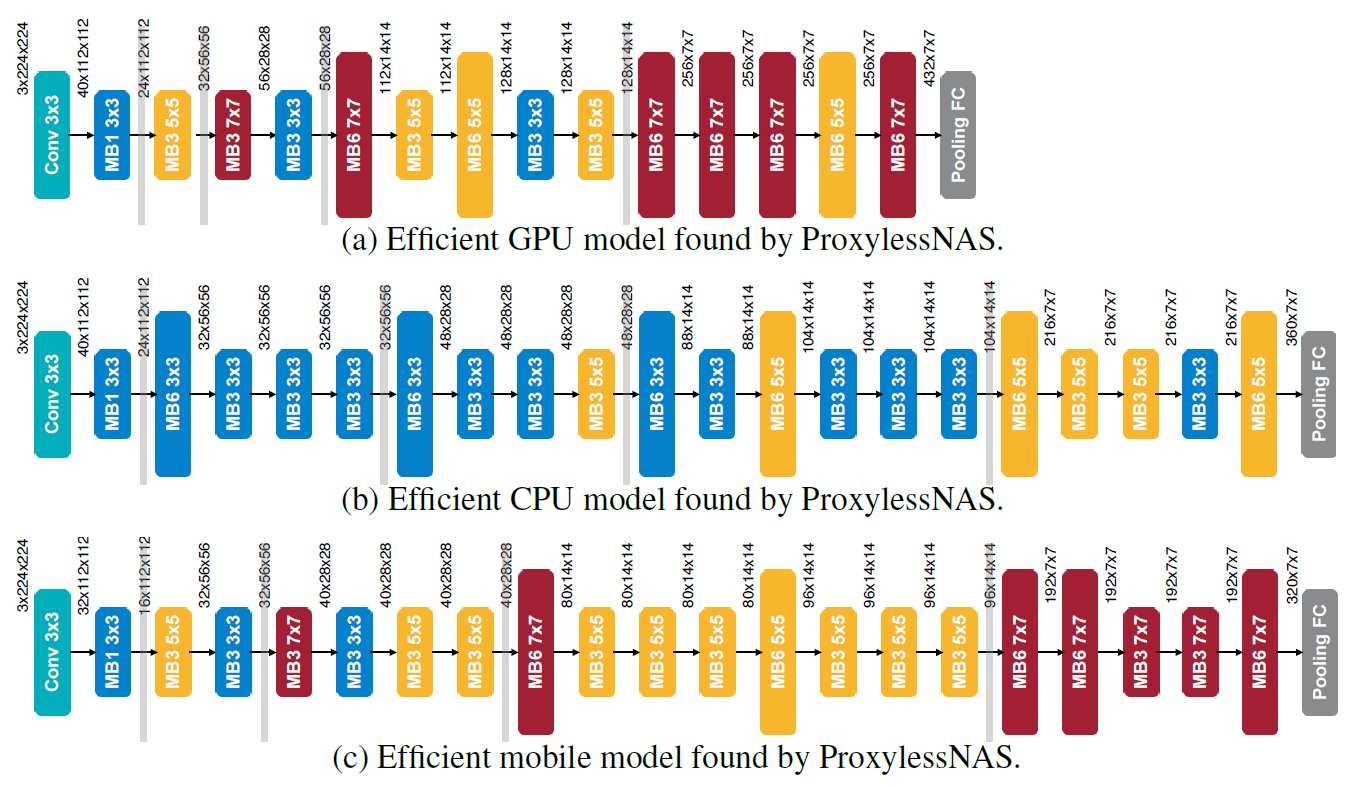
\includegraphics[width=.85\columnwidth]{../../../img/proxylessnas.png}
\end{center}

\begin{center}
\scriptsize{ProxylessNAS: Direct Neural Architecture Search on Target Task and Hardware (ICLR 2019)}
\end{center}
\end{frame}

\begin{frame}[label={sec:org987ef14}]{Neural Architecture Search}
\begin{center}
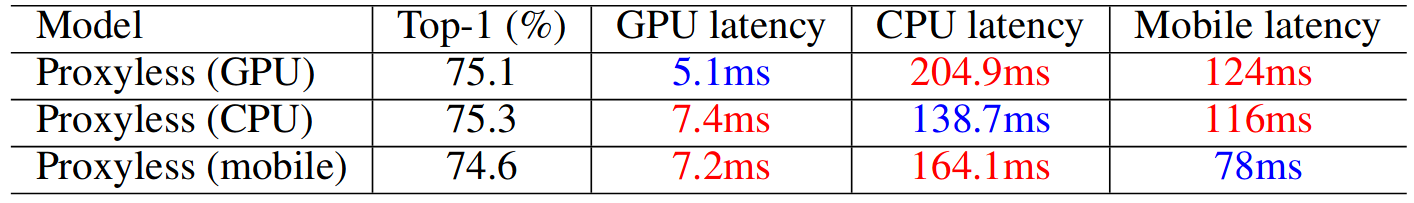
\includegraphics[width=.75\columnwidth]{../../../img/proxylessnas_II.png}
\end{center}

\begin{center}
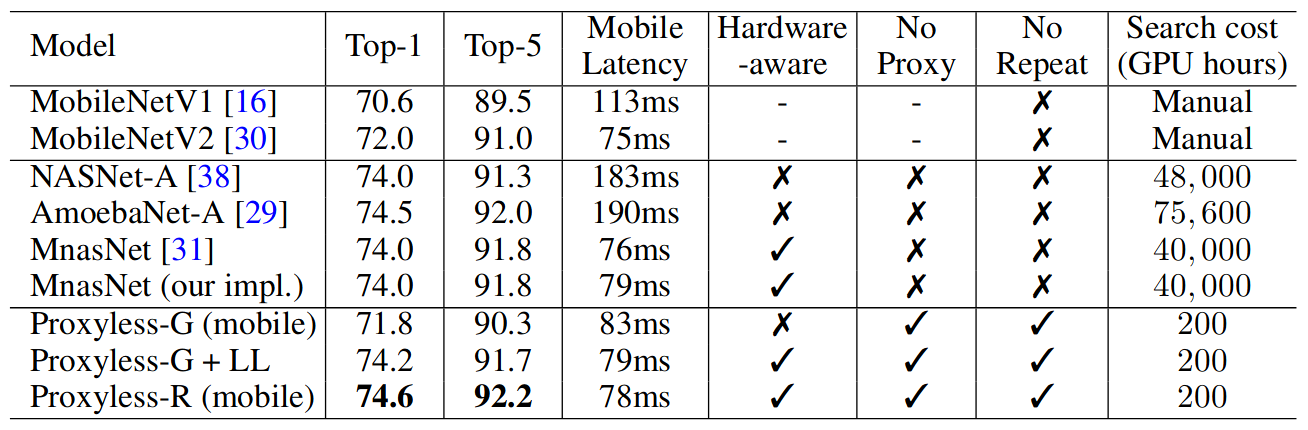
\includegraphics[width=.85\columnwidth]{../../../img/proxylessnas_I.png}
\end{center}

\begin{center}
\scriptsize{ProxylessNAS: Direct Neural Architecture Search on Target Task and Hardware (ICLR 2019)}
\end{center}
\end{frame}
\maketitle
\end{document}
